\documentclass[12pt]{article}
\usepackage{amsmath,amssymb,amsthm}
\usepackage{geometry}
\geometry{margin=1in}
\usepackage{graphicx}
\usepackage{cite}
\usepackage{float}

\title{Report 3}
\author{Yaghoub Shahmari}
\date{\today}

\begin{document}
\maketitle

\begin{abstract}
In this report, we present a generalized model for malaria transmission that extends the classical Ross-Macdonald framework by incorporating an arbitrary number of latent stages in mosquito populations using an Erlang distribution. Both untreated and treated mosquito populations are assumed to have multiple latent compartments, with treatment coupling incorporated through an additional transition. We derive the general form of the underlying ordinary differential equations (ODEs) and present the structure of the corresponding New Infections (\(F\)) and Transition (\(V\)) matrices used in the Next Generation Matrix (NGM) method for computing the basic reproduction number, \(R_0\). We also discuss the analytical form of the endemic equilibrium, showing that while closed-form expressions exist for each compartment in terms of the infected human fraction, the consistency condition for the human equilibrium results in a nonlinear equation that generally must be solved numerically.
\end{abstract}

\section{Introduction}
Mathematical models for malaria transmission have traditionally followed the Ross-Macdonald framework, compartmentalizing both the human and mosquito populations. Most previous works have assumed two latent stages in the mosquito dynamics. In order to capture the observed variance in the latent period and to allow for more flexibility, we generalize the model to allow an arbitrary number of latent compartments following an Erlang distribution. In the generalized model we denote:
\begin{itemize}
  \item \(N_{LM}\): Number of latent stages for untreated mosquitoes.
  \item \(N_{LT}\): Number of latent stages for treated mosquitoes.
\end{itemize}
The progression rates through the latent stages are denoted \(s_M\) for untreated mosquitoes and \(s_T\) for treated mosquitoes. This extension allows us to explore in greater detail the impact of the latent period distribution on the basic reproduction number and endemic state.

\section{Model Formulation}

\subsection{Compartments and Notation}
The model divides the populations as follows:
\begin{enumerate}
    \item \textbf{Humans:} Two compartments are considered:
    \[
    S_H \quad \text{(susceptible)}, \quad I_H \quad \text{(infected)},
    \]
    with the normalization \(S_H + I_H = 1\).
    
    \item \textbf{Untreated Mosquitoes:} These are subdivided into:
    \[
    S_M,\; E_{1,M},\, E_{2,M},\, \dots,\, E_{N_{LM},M},\; I_M,
    \]
    where \(S_M\) is the susceptible class, \(E_{i,M}\) (\(i=1,\dots,N_{LM}\)) are the latent compartments, and \(I_M\) is the infectious class.
    
    \item \textbf{Treated Mosquitoes:} Similarly, these are subdivided into:
    \[
    S_T,\; E_{1,T},\, E_{2,T},\, \dots,\, E_{N_{LT},T},\; I_T.
    \]
\end{enumerate}

The equilibrium values of the susceptible mosquito classes \(S_M\) and \(S_T\) at the disease-free equilibrium (DFE) are obtained by solving the linear system
\[
\begin{pmatrix}
-(t+g) & h \\
t       & -(h+g)
\end{pmatrix}
\begin{pmatrix}
S^*_M \\ S^*_T
\end{pmatrix}
=
\begin{pmatrix}
-g \\ 0
\end{pmatrix},
\]
where \(g\) is the mosquito death rate, \(h\) is the treatment waning rate, and \(t\) is the treatment encounter rate.

\subsection{Generalized ODE Model}
The dynamics of the system are governed by the following sets of ODEs.

\paragraph{Humans (SIS model):}
\begin{align}
\frac{dS_H}{dt} &= - m a b (I_M + I_T) S_H + r I_H, \\
\frac{dI_H}{dt} &= m a b (I_M + I_T) S_H - r I_H,
\end{align}
where:
\begin{itemize}
    \item \(a\) is the biting rate,
    \item \(b\) is the probability of transmission from mosquito to human,
    \item \(m\) is the mosquito-to-human ratio,
    \item \(r\) is the human recovery rate.
\end{itemize}

\paragraph{Untreated Mosquitoes:}
\begin{align}
\frac{dS_M}{dt} &= g + h S_T - a c I_H S_M - tS_M - gS_M, \\
\frac{dE_{1,M}}{dt} &= a c I_H S_M - \Big( t + s_M + g \Big) E_{1,M}, \\
\frac{dE_{i,M}}{dt} &= s_M E_{i-1,M} - (s_M+g) E_{i,M}, \quad i=2,\dots,N_{LM}, \\
\frac{dI_M}{dt} &= s_M E_{N_{LM},M} - g I_M.
\end{align}

\paragraph{Treated Mosquitoes:}
\begin{align}
\frac{dS_T}{dt} &= t S_M - a c I_H S_T - h S_T - g S_T, \\
\frac{dE_{1,T}}{dt} &= a c I_H S_T + tE_{1,M} - (s_T + g) E_{1,T}, \\
\frac{dE_{i,T}}{dt} &= s_T E_{i-1,T} - (s_T+g)E_{i,T}, \quad i=2,\dots,N_{LT}, \\
\frac{dI_T}{dt} &= s_T E_{N_{LT},T} - g I_T.
\end{align}

The term \(tE_{1,M}\) in the equation for \(E_{1,T}\) reflects that some mosquitoes in the untreated latent compartment are transferred to the treated branch upon treatment encounter.

\section{Next Generation Matrix and Calculation of \(R_0\)}

\subsection{Infected Compartments and Matrix Structure}
We define the vector of infected compartments as
\[
\mathbf{x} = \begin{bmatrix}
I_H,\, E_{1,M},\, \dots,\, E_{N_{LM},M},\, I_M,\, E_{1,T},\, \dots,\, E_{N_{LT},T},\, I_T
\end{bmatrix}^\top.
\]
The total number of infected compartments is:
\[
n_{\text{inf}} = 1 + (N_{LM}+1) + (N_{LT}+1).
\]

\subsection{New Infections Matrix \(\mathbf{F}\)}
New infections arise as follows:
\begin{itemize}
    \item Humans become infected from bites by infectious mosquitoes:
    \[
    F_{1, I_M} = m a b S_H^*, \quad F_{1, I_T} = m a b S_H^*.
    \]
    \item Mosquitoes become infected when biting an infectious human. New infections appear in the first latent compartment of each branch:
    \[
    F_{E_{1,M}, I_H} = a c S_M^*, \quad F_{E_{1,T}, I_H} = a c S_T^*.
    \]
\end{itemize}
All other entries of \(\mathbf{F}\) are zero.

\subsection{Transition Matrix \(\mathbf{V}\)}
The matrix \(\mathbf{V}\) represents the departures from each compartment due to progression, treatment, recovery, or death.
\begin{itemize}
    \item \textbf{Humans:} 
    \[
    V_{1,1} = r.
    \]
    
    \item \textbf{Untreated Mosquitoes:}
    \begin{align*}
    V_{E_{1,M},E_{1,M}} &= t+ s_M + g,\\[1mm]
    V_{E_{i,M},E_{i,M}} &= s_M + g, \quad V_{E_{i,M},E_{i-1,M}} = - s_M, \quad i=2,\dots,N_{LM},\\[1mm]
    V_{I_M,I_M} &= g, \quad V_{I_M,E_{N_{LM},M}} = - s_M.
    \end{align*}
    
    \item \textbf{Treated Mosquitoes:}
    \begin{align*}
    V_{E_{1,T},E_{1,T}} &= s_T + g, \quad \text{with an additional transfer term }V_{E_{1,T},E_{1,M}} = -t,\\[1mm]
    V_{E_{i,T},E_{i,T}} &= s_T + g, \quad V_{E_{i,T},E_{i-1,T}} = - s_T, \quad i=2,\dots,N_{LT},\\[1mm]
    V_{I_T,I_T} &= g, \quad V_{I_T,E_{N_{LT},T}} = - s_T.
    \end{align*}
\end{itemize}

The Next Generation Matrix is then given by
\[
\mathbf{NGM} = \mathbf{F} \mathbf{V}^{-1},
\]
and the basic reproduction number is
\[
R_0 = \rho(\mathbf{NGM}),
\]
where \(\rho\) denotes the spectral radius (largest eigenvalue).

\section{Analytical Derivation of the Endemic Equilibrium}
At endemic equilibrium all derivatives are zero. For the human host dynamics (using an SIS model), we have:
\begin{equation}
\frac{I_H}{1-I_H} = \frac{m\,a\,b\,(I_M+I_T)}{r}.
\end{equation}

\subsection{Analytical Expressions for Mosquito Compartments}
Using the ODE balance equations in equilibrium, we derive the following analytical expressions:
\begin{itemize}
    \item \textbf{Untreated Mosquitoes:}
    \begin{align}
    E_{1,M} &= \frac{a\,c\,I_H\,S_M}{t + s_M + g},\\[1mm]
    E_{i,M} &= \left(\frac{s_M}{s_M+g}\right)^{i-1}E_{1,M}, \quad i=2,\dots, N_{LM},\\[1mm]
    I_M &= \frac{s_M}{g}\left(\frac{s_M}{s_M+g}\right)^{N_{LM}-1}E_{1,M}.
    \end{align}
    
    \item \textbf{Treated Mosquitoes:}
    \begin{align}
    S_T &= \frac{t\,S_M}{a\,c\,I_H + h + g},\\[1mm]
    E_{1,T} &= \frac{a\,c\,I_H\,S_T + tE_{1,M}}{s_T + g},\\[1mm]
    E_{i,T} &= \left(\frac{s_T}{s_T+g}\right)^{i-1}E_{1,T}, \quad i=2,\dots, N_{LT},\\[1mm]
    I_T &= \frac{s_T}{g}\left(\frac{s_T}{s_T+g}\right)^{N_{LT}-1}E_{1,T}.
    \end{align}
\end{itemize}

In these expressions the equilibrium value \(S_M\) for untreated susceptible mosquitoes is derived from their balance at the DFE (modified by the impact of infection), and \(S_T\) is expressed in terms of \(S_M\).

\subsection{Consistency Condition for \(I_H\)}
By substituting the analytical expressions for \(I_M\) and \(I_T\) into the human equilibrium condition, we obtain a consistency equation:
\[
\frac{I_H}{1-I_H} = \frac{m\,a\,b\,\left[I_M(I_H)+I_T(I_H)\right]}{r},
\]
in which \(I_M\) and \(I_T\) are given by the formulas above as functions of \(I_H\) (and implicitly, \(S_M\) and \(S_T\)). For the simplest case (e.g. \(N_{LM}=N_{LT}=2\)) this consistency equation is quadratic in \(I_H\) and can be solved in closed form. However, for an arbitrary number of latent stages the equation becomes a polynomial of higher degree (or even transcendental) and generally cannot be solved by radicals. Thus, although the system has an analytical structure, the final determination of \(I_H\) typically requires a numerical solution of the consistency equation.

\section{Results}

\subsection{R0 for treatment rate/period parameters}

\begin{figure}[H]
    \centering
    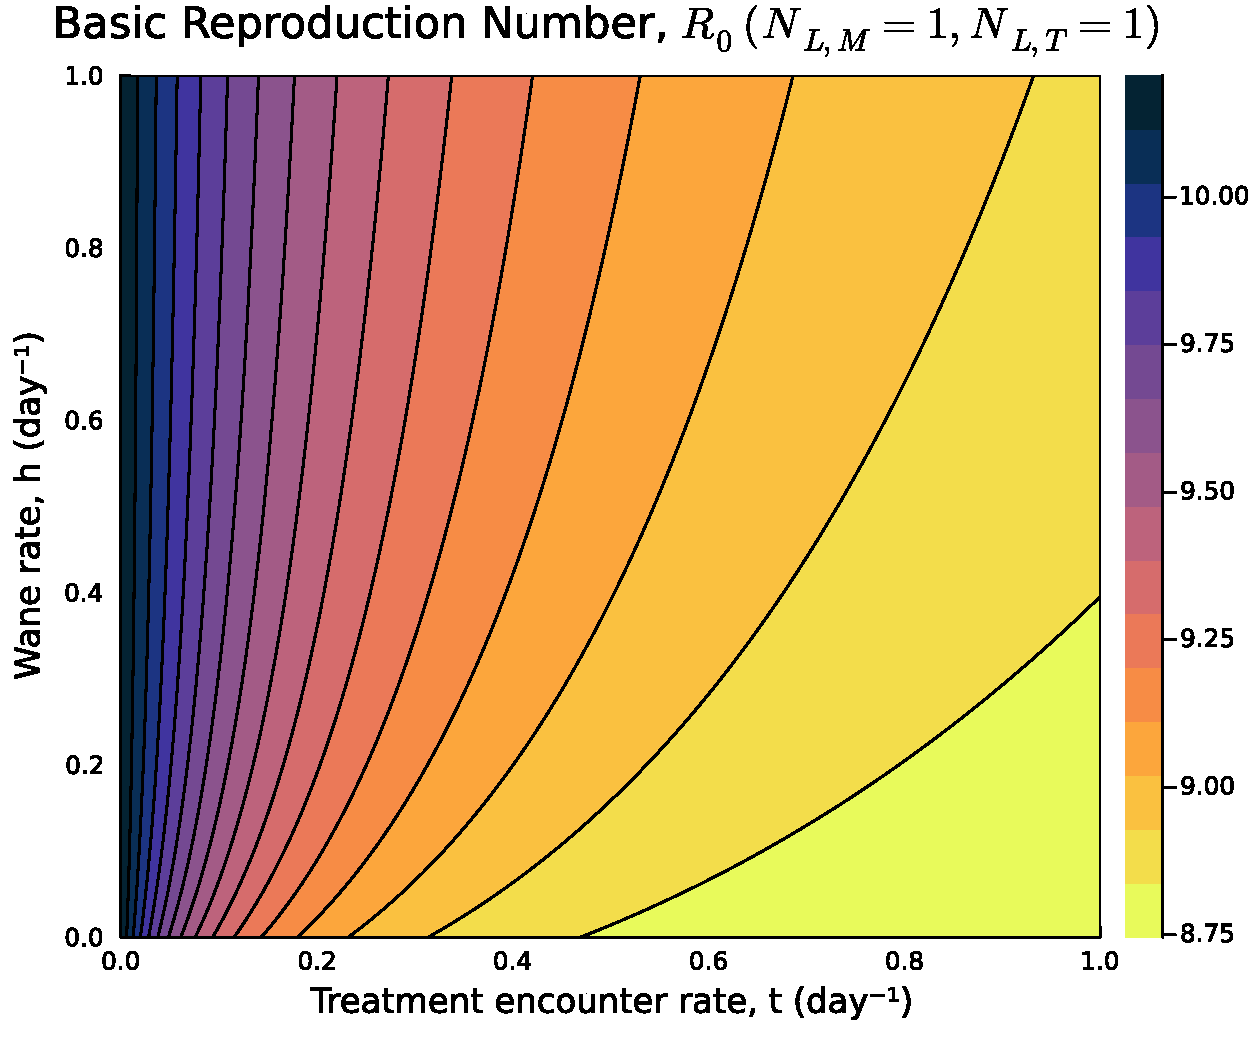
\includegraphics[width=0.3\textwidth]{../../fig/gen_model/R0_rates_txh_1x1.pdf}
    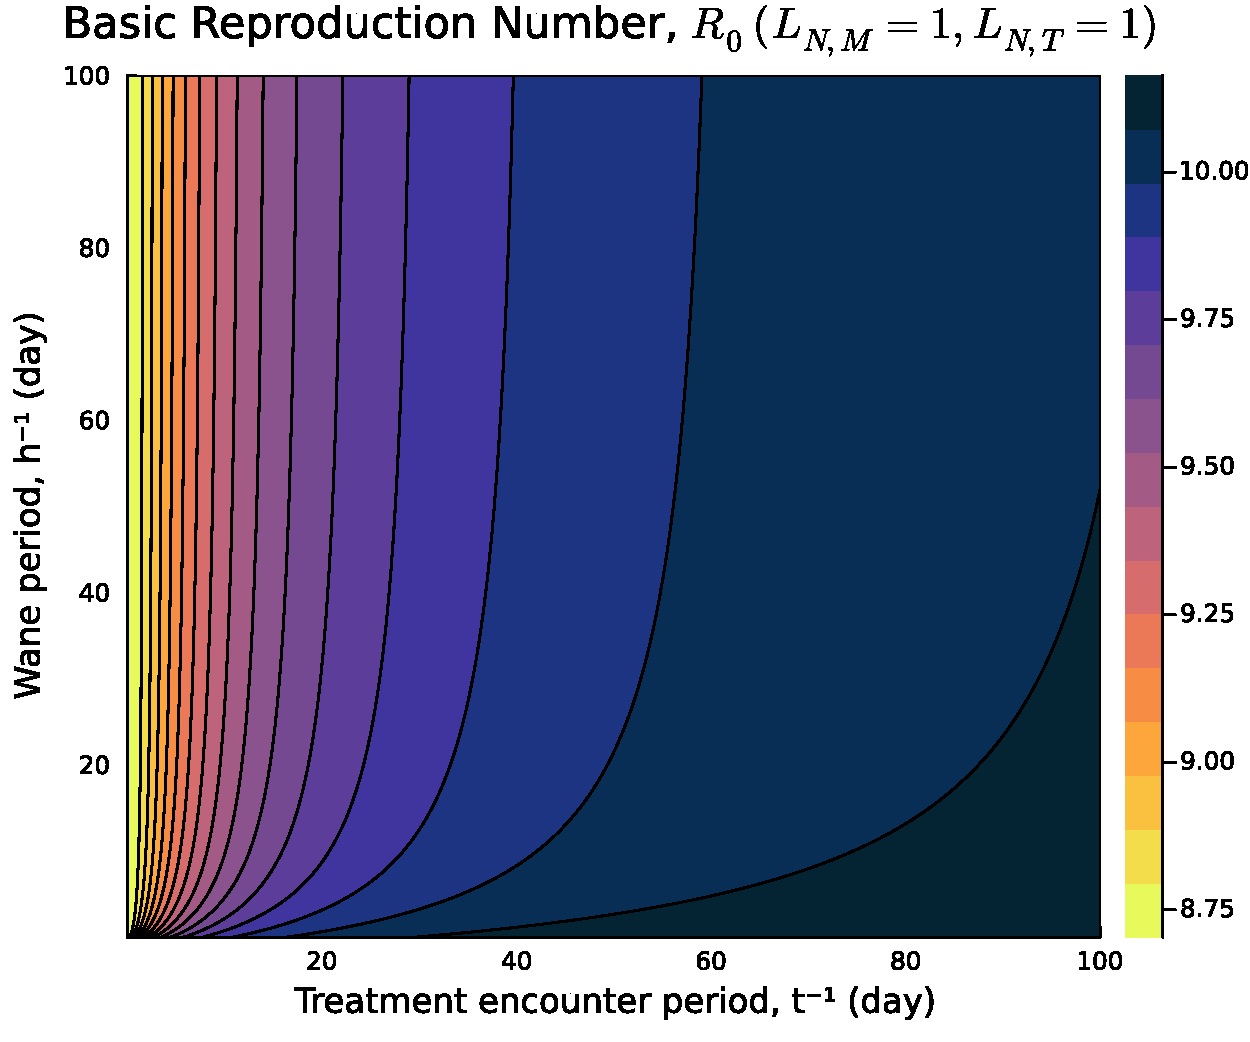
\includegraphics[width=0.3\textwidth]{../../fig/gen_model/R0_periods_txh_1x1.pdf}\\
    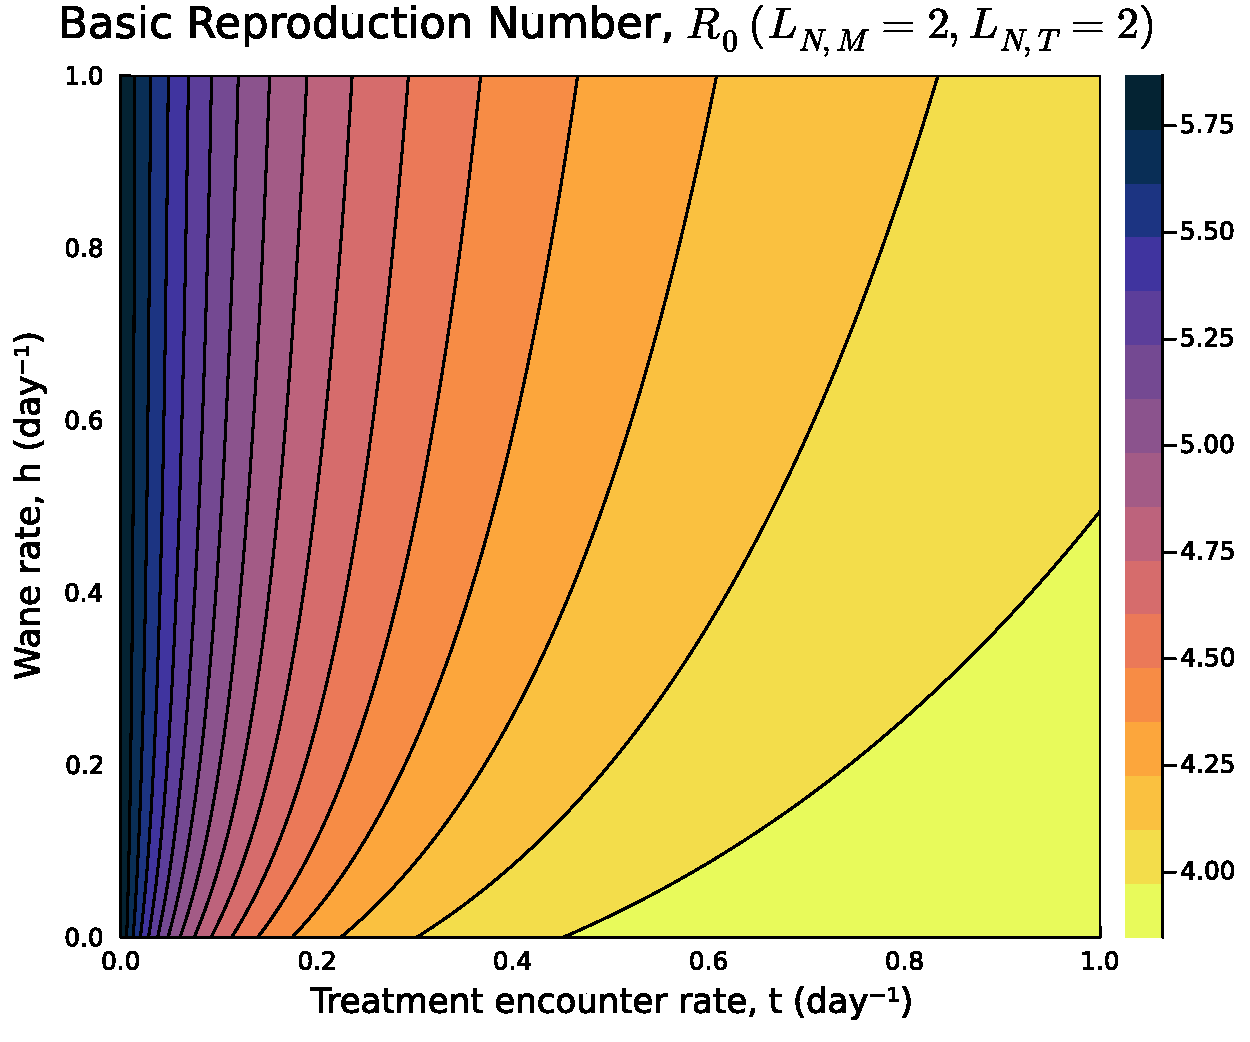
\includegraphics[width=0.3\textwidth]{../../fig/gen_model/R0_rates_txh_2x2.pdf}
    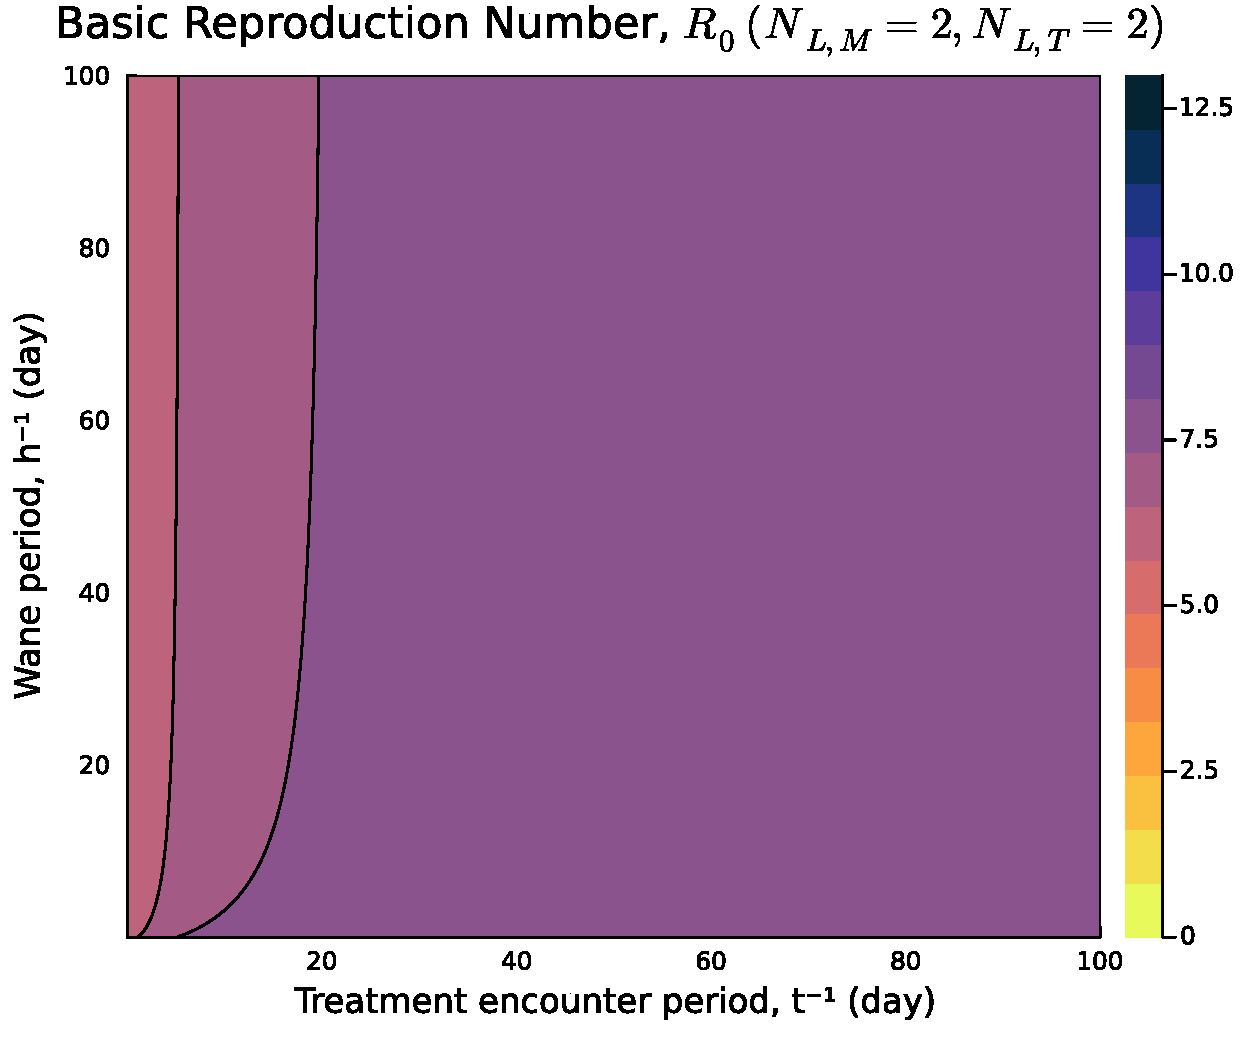
\includegraphics[width=0.3\textwidth]{../../fig/gen_model/R0_periods_txh_2x2.pdf}\\
    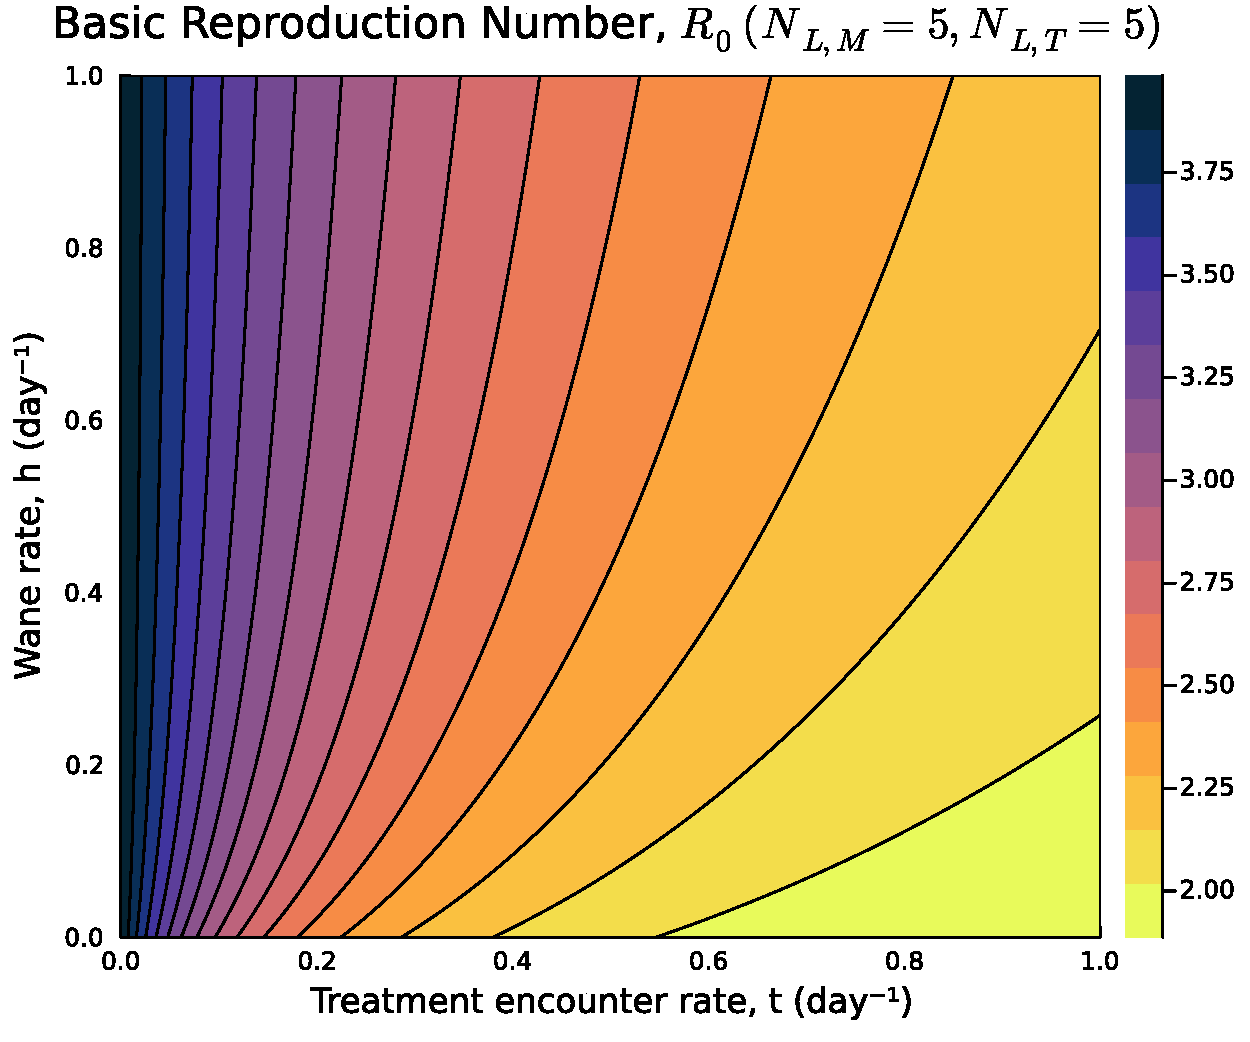
\includegraphics[width=0.3\textwidth]{../../fig/gen_model/R0_rates_txh_5x5.pdf}
    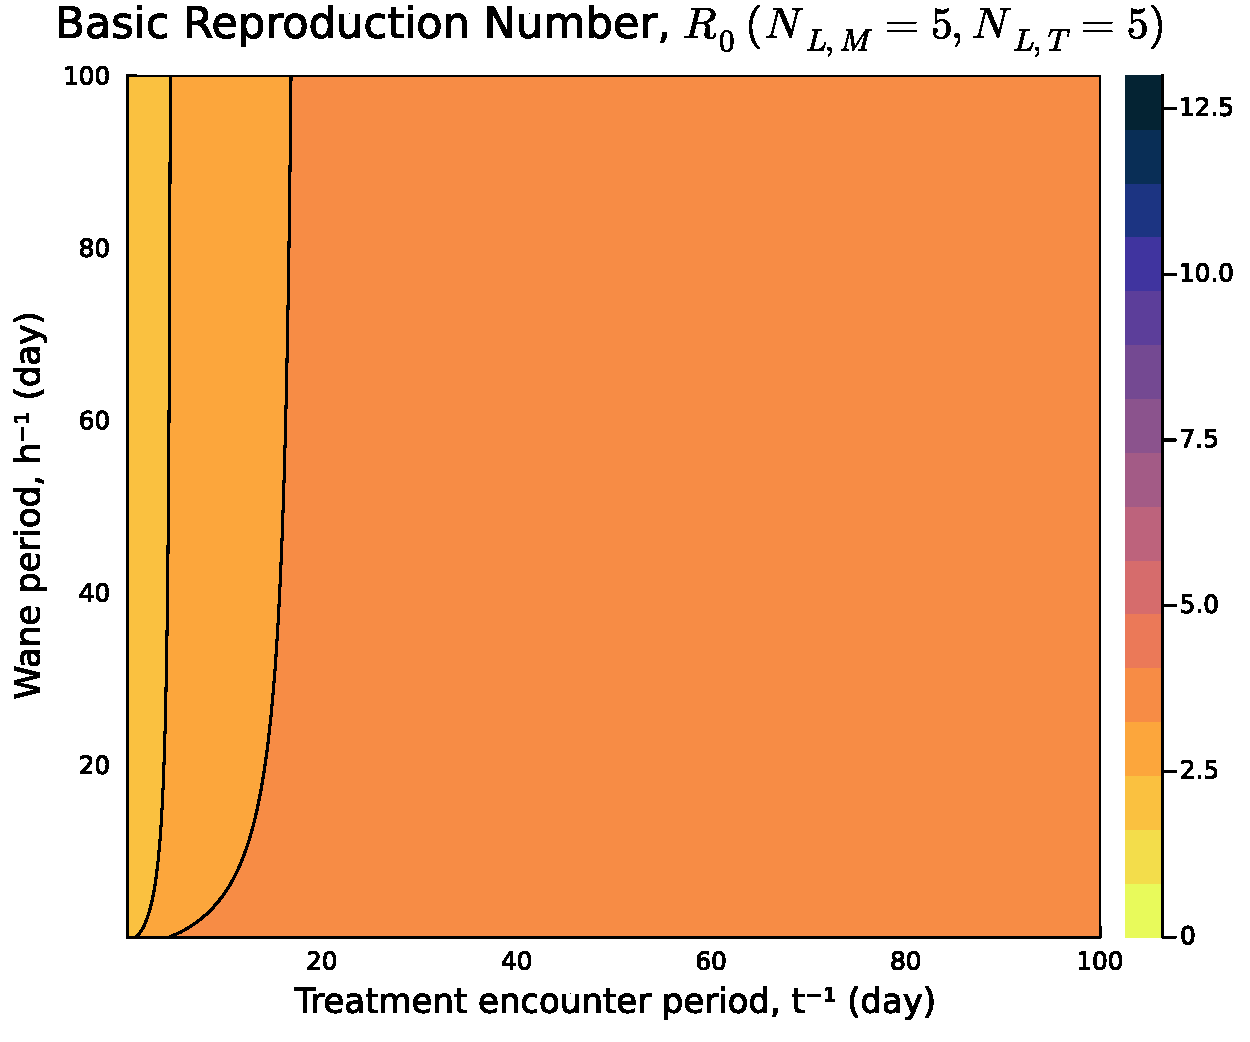
\includegraphics[width=0.3\textwidth]{../../fig/gen_model/R0_periods_txh_5x5.pdf}\\
    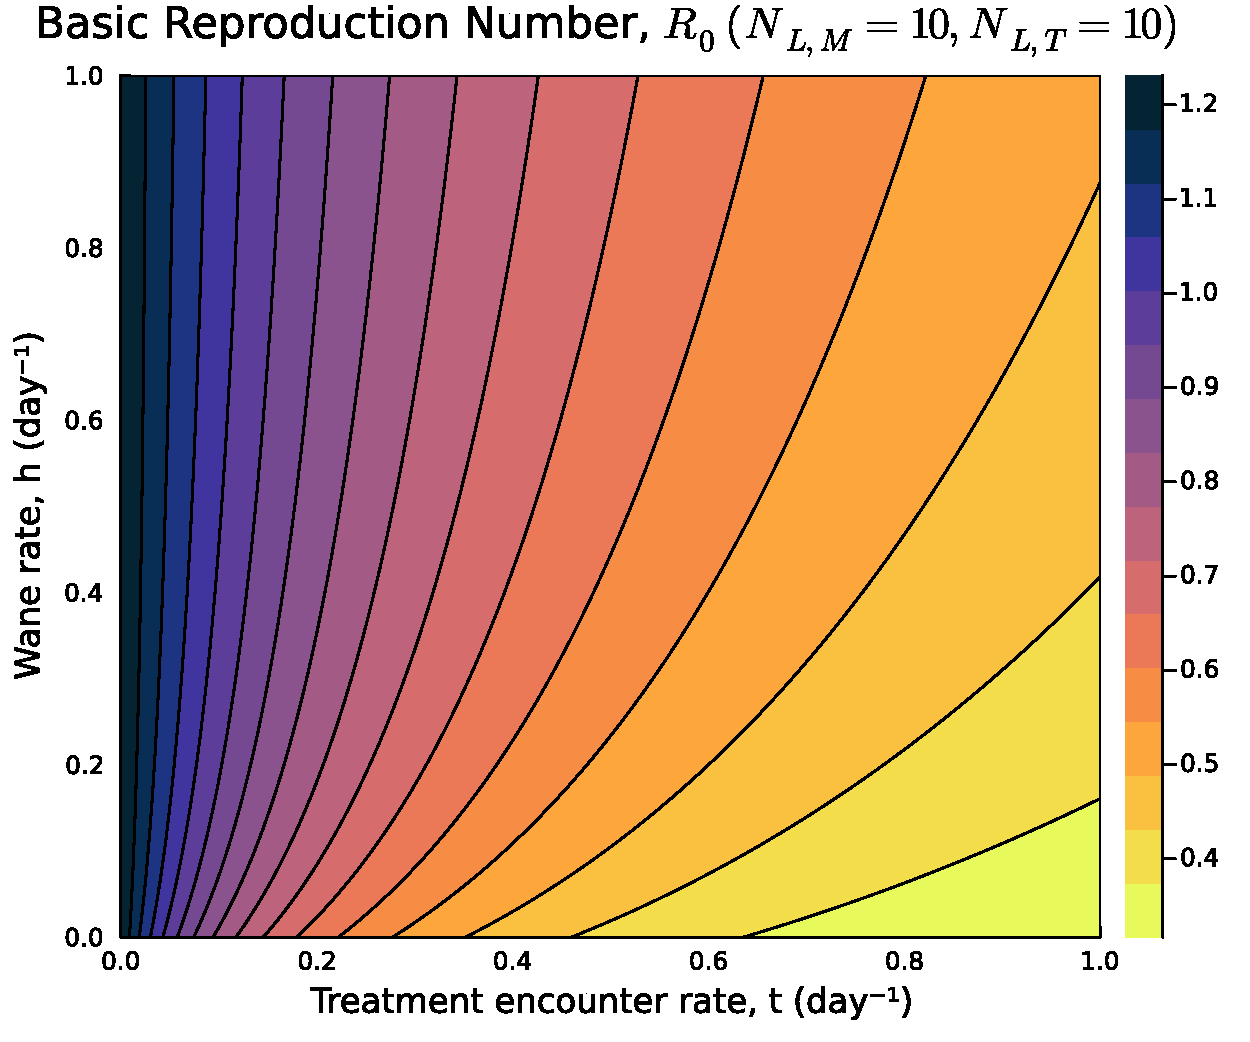
\includegraphics[width=0.3\textwidth]{../../fig/gen_model/R0_rates_txh_10x10.pdf}
    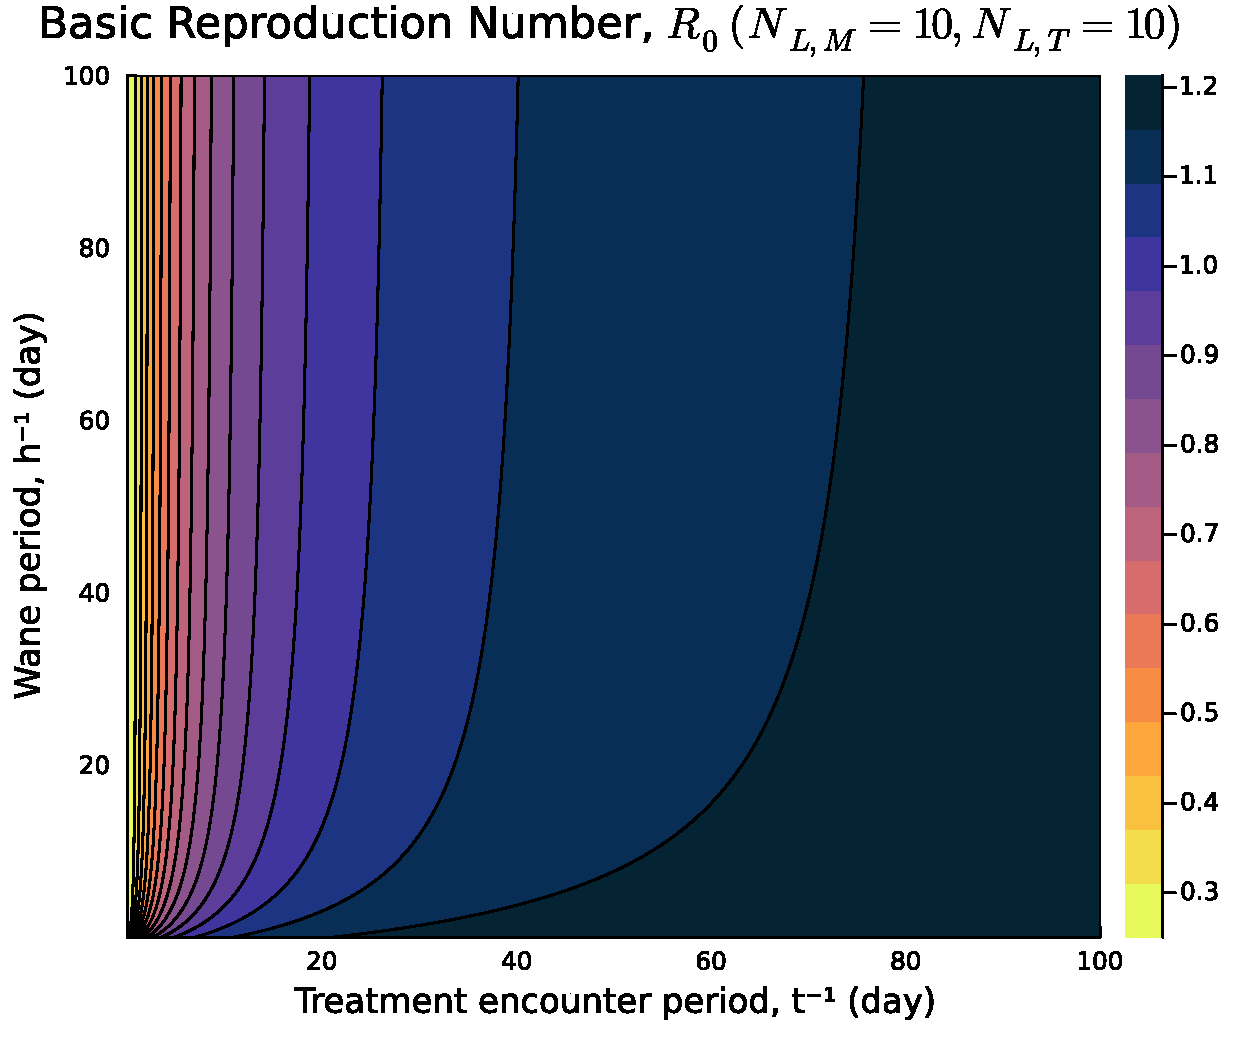
\includegraphics[width=0.3\textwidth]{../../fig/gen_model/R0_periods_txh_10x10.pdf}
    \caption{\textbf{R0 for treatment rate/period parameters.} The left panels shows the basic reproduction number \(R_0\) as a function of the treatment rate, while the right panels shows \(R_0\) as a function of the treatment period.}
\end{figure}

\begin{figure}[H]
    \centering
    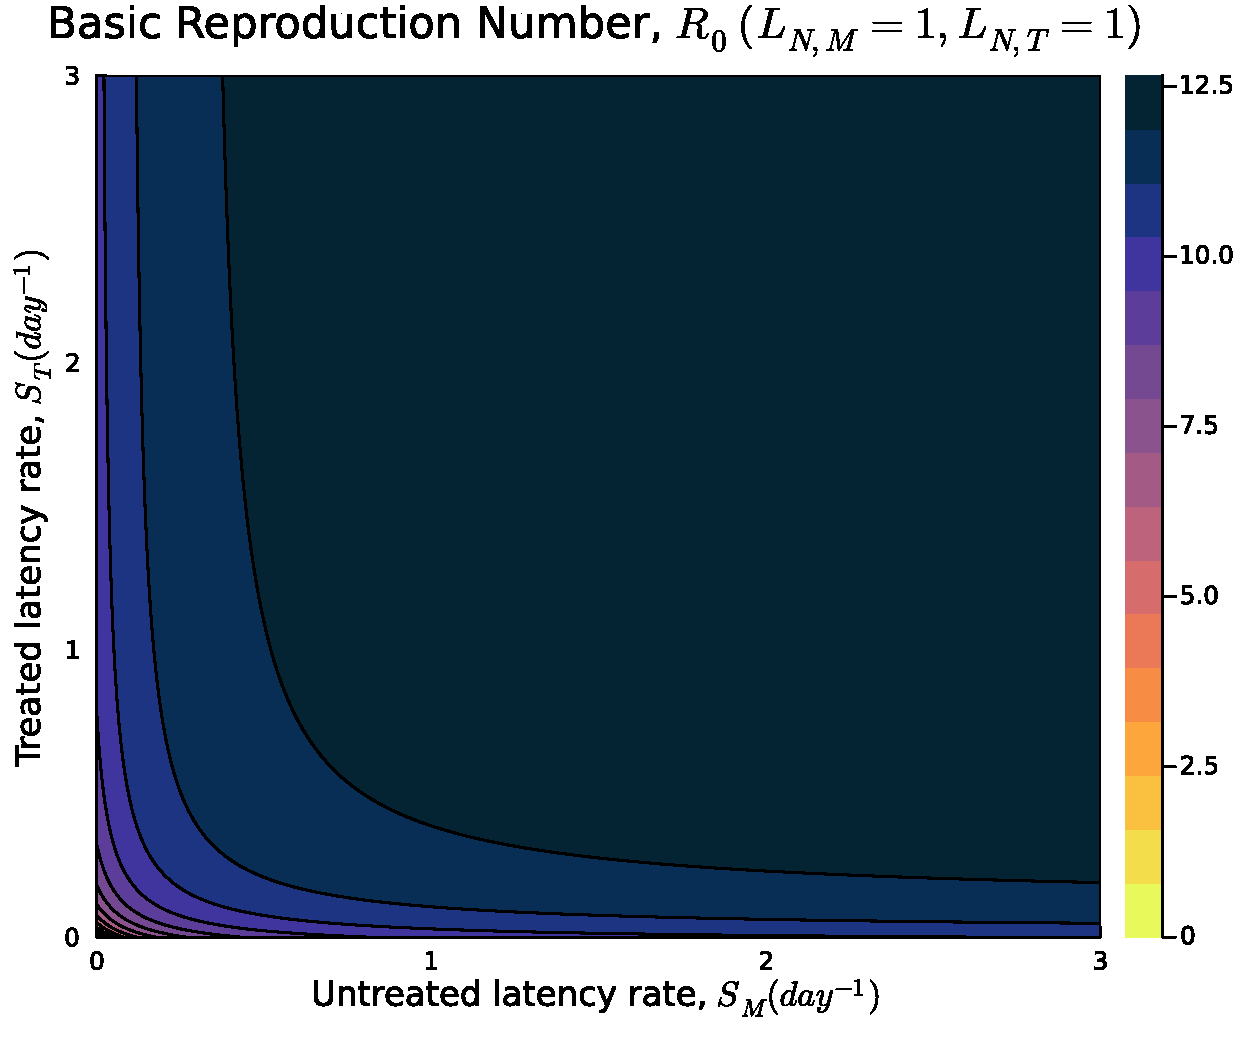
\includegraphics[width=0.3\textwidth]{../../fig/gen_model/R0_rates_SMxST_1x1.pdf}
    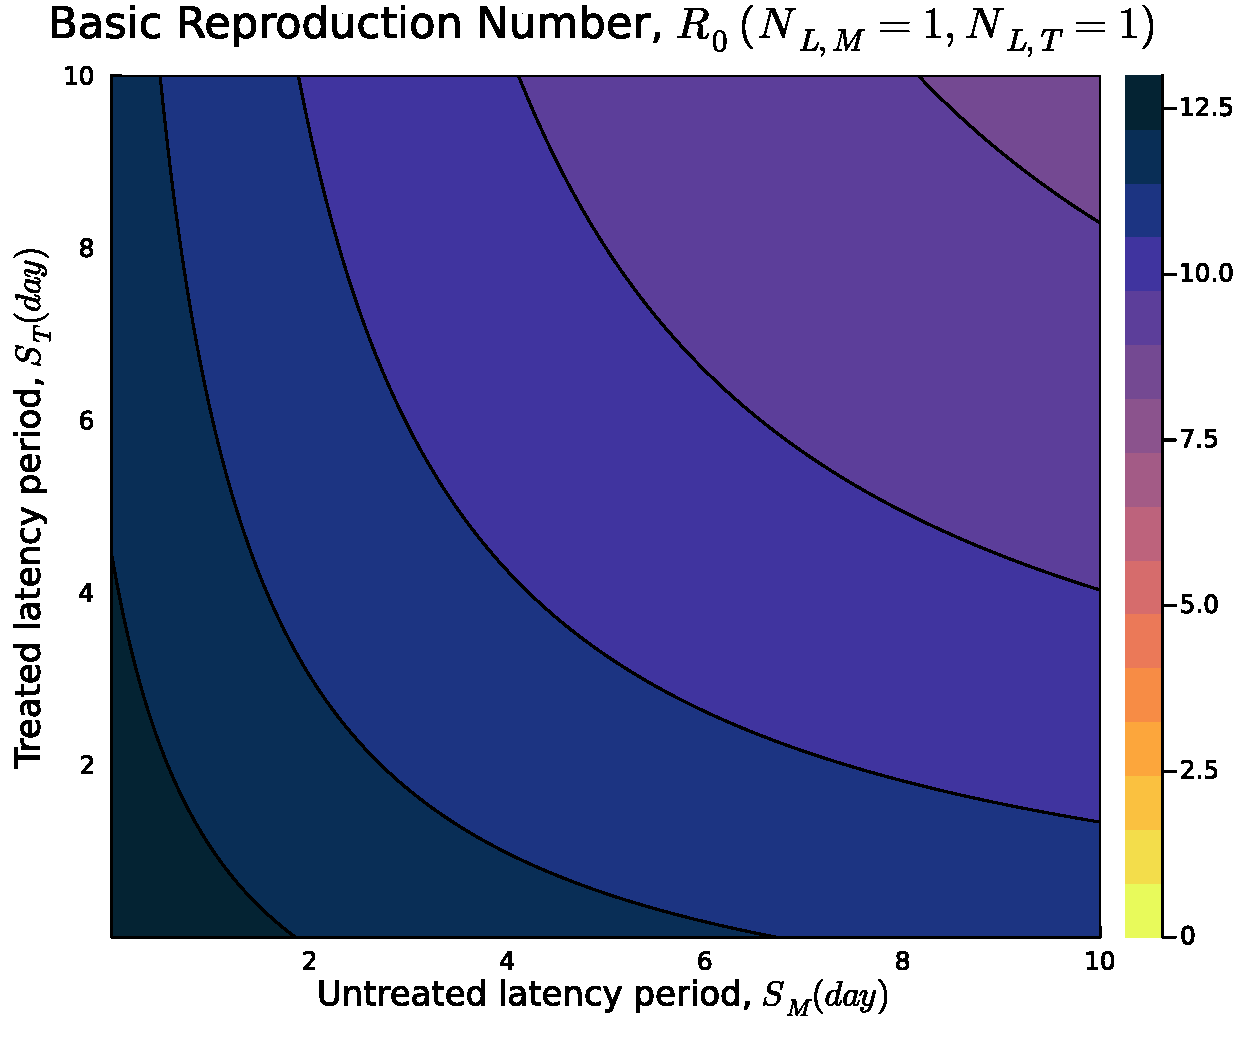
\includegraphics[width=0.3\textwidth]{../../fig/gen_model/R0_periods_SMxST_1x1.pdf}\\
    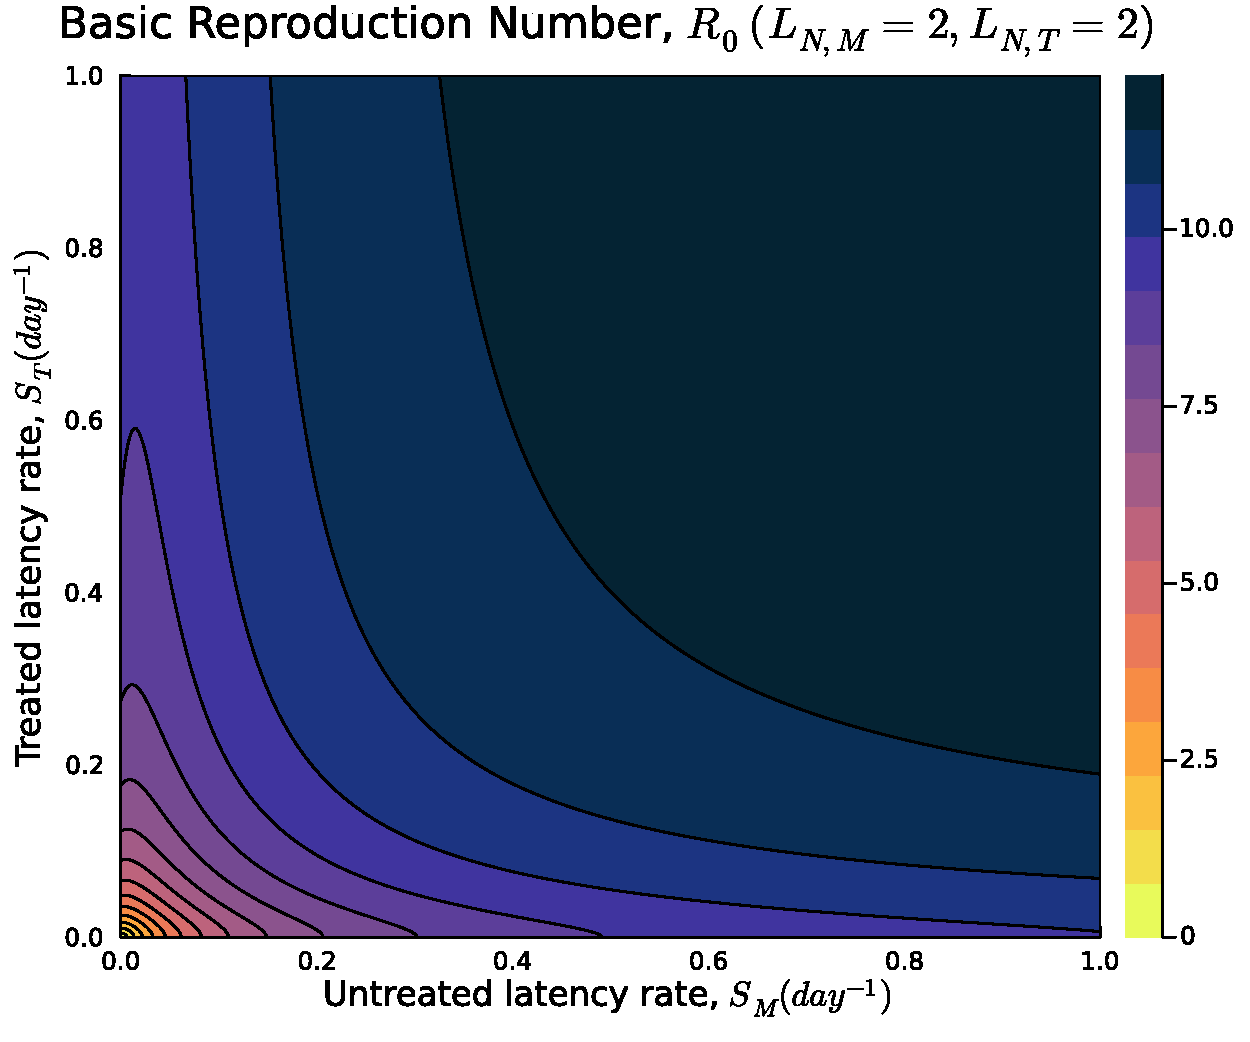
\includegraphics[width=0.3\textwidth]{../../fig/gen_model/R0_rates_SMxST_2x2.pdf}
    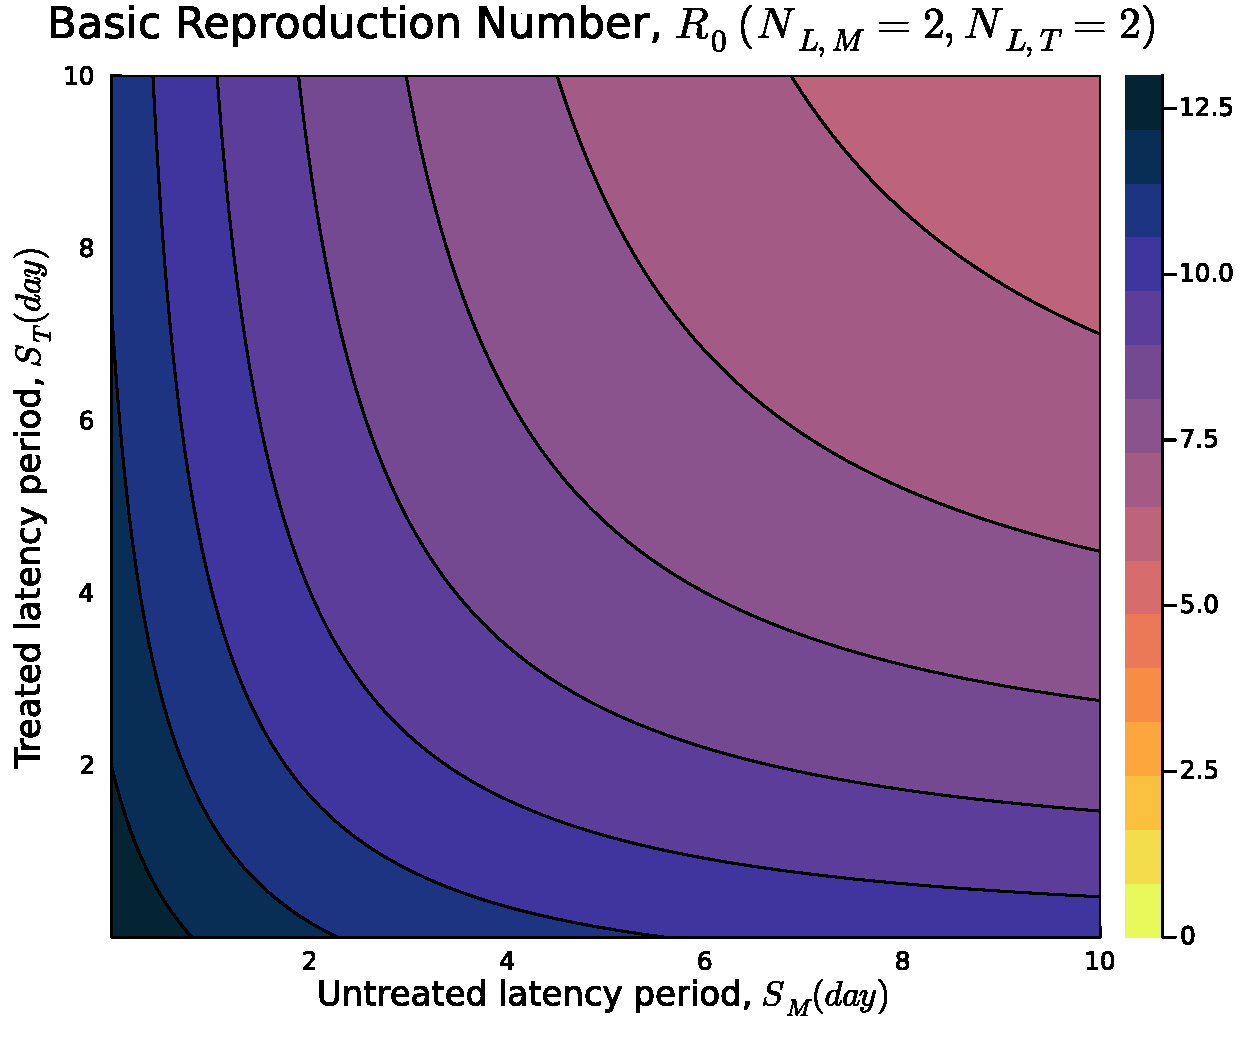
\includegraphics[width=0.3\textwidth]{../../fig/gen_model/R0_periods_SMxST_2x2.pdf}\\
    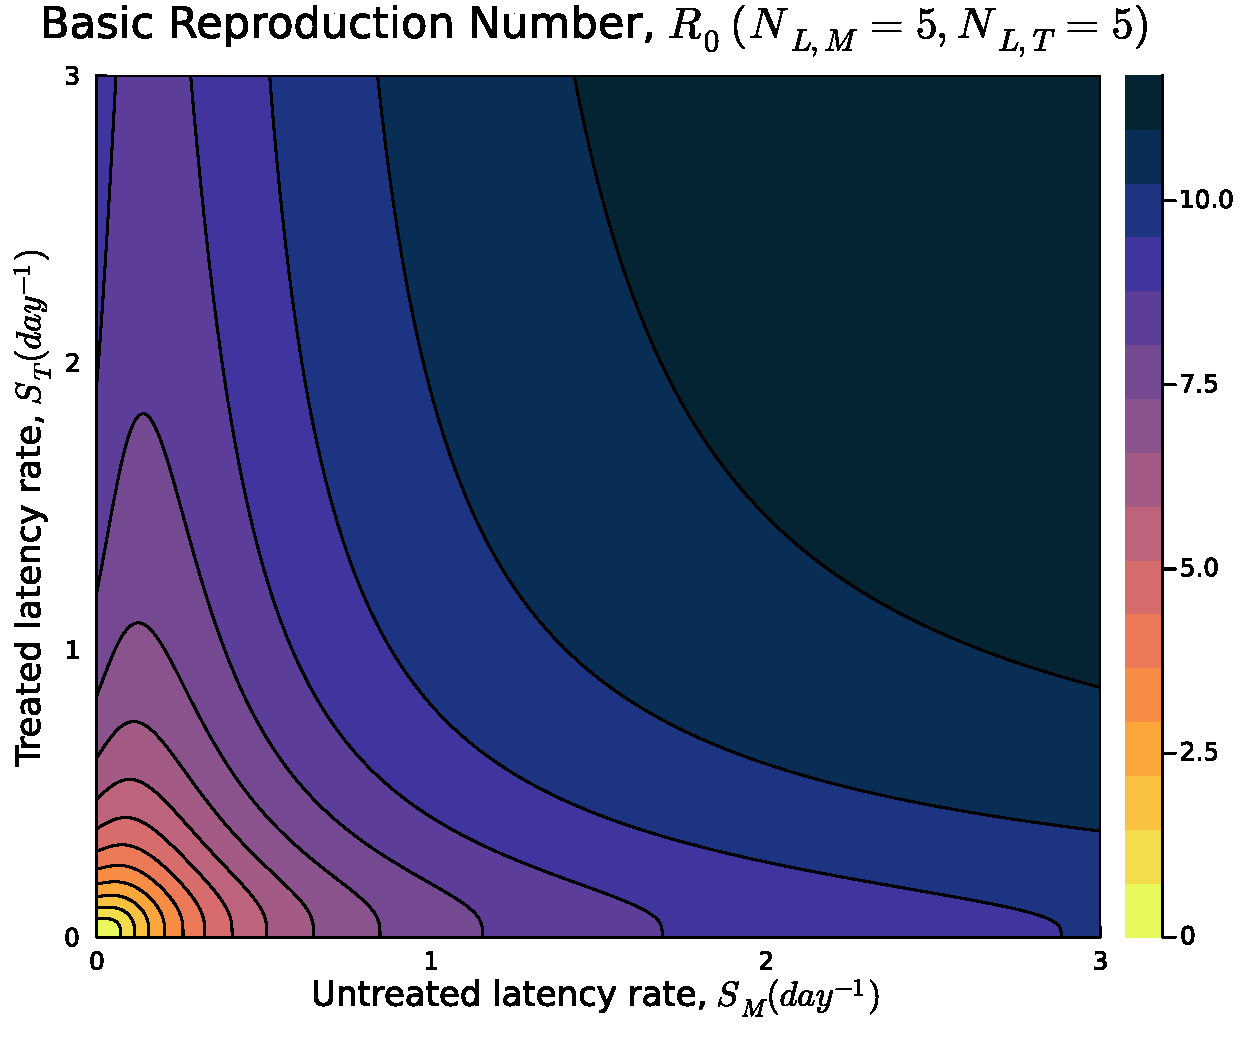
\includegraphics[width=0.3\textwidth]{../../fig/gen_model/R0_rates_SMxST_5x5.pdf}
    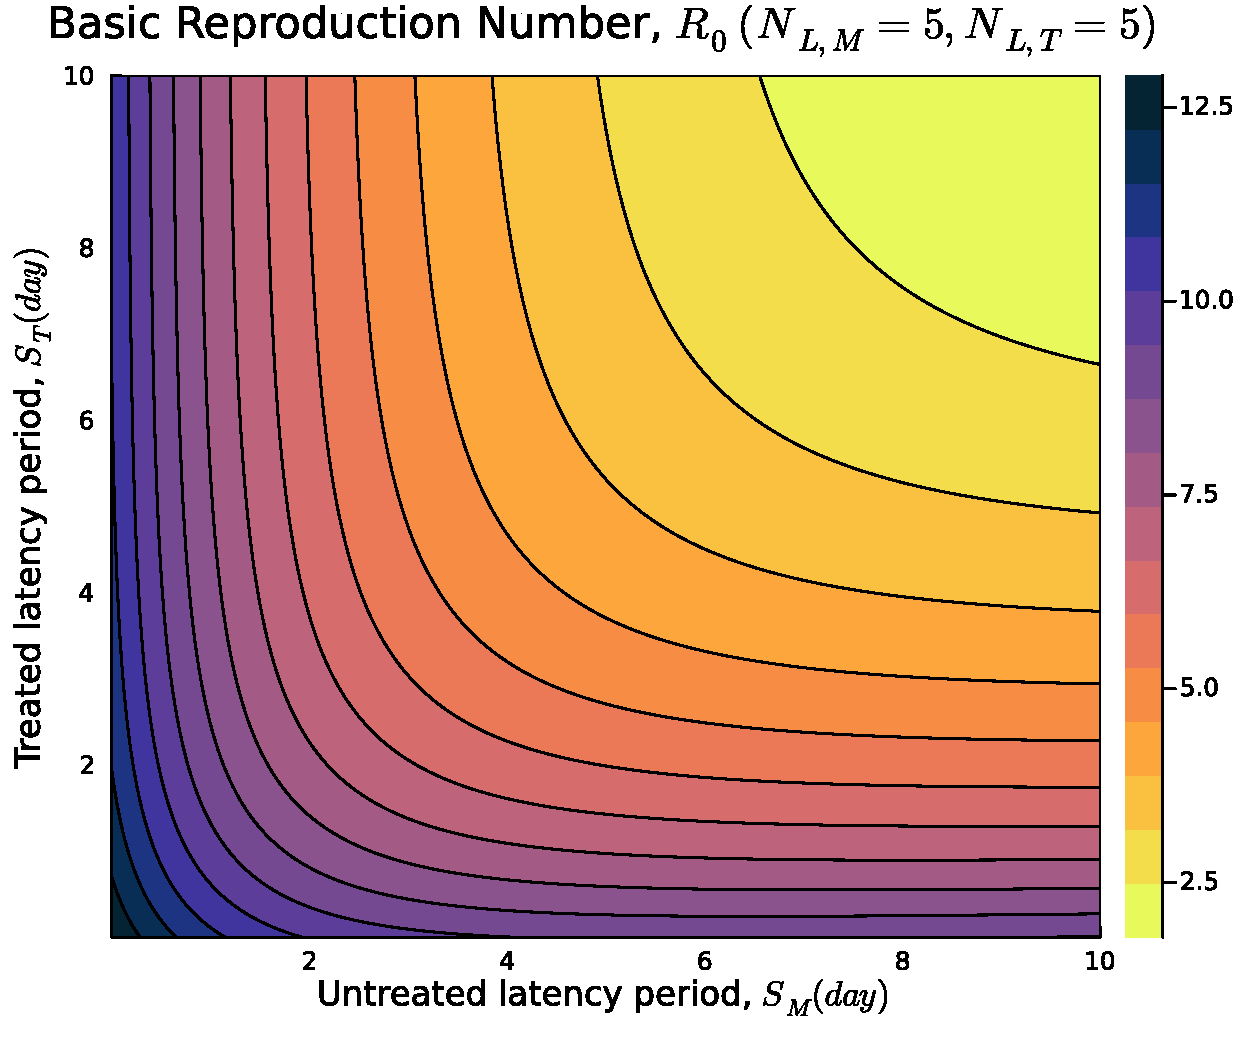
\includegraphics[width=0.3\textwidth]{../../fig/gen_model/R0_periods_SMxST_5x5.pdf}\\
    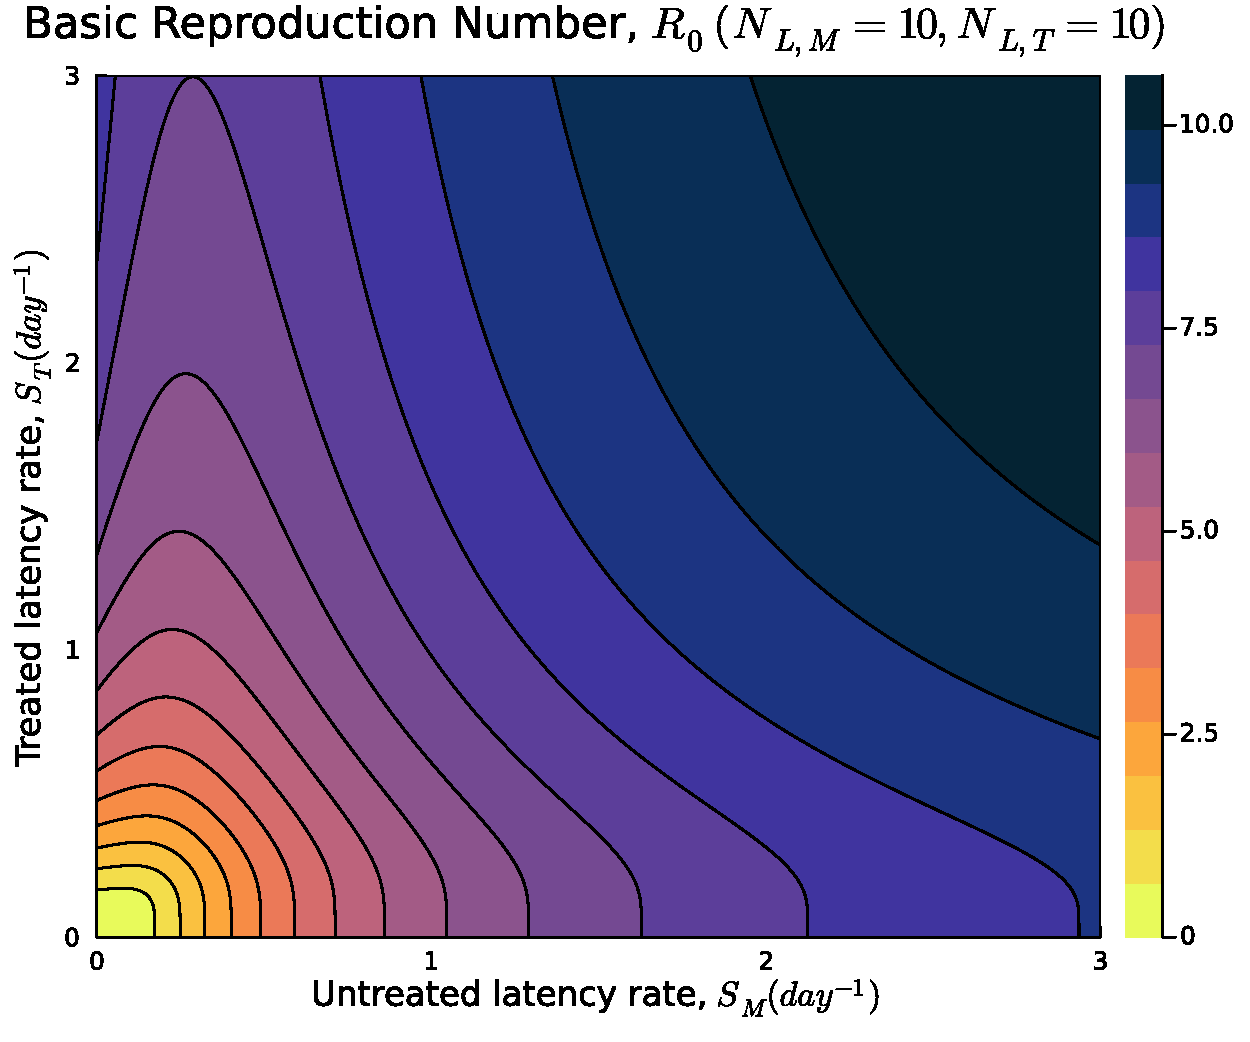
\includegraphics[width=0.3\textwidth]{../../fig/gen_model/R0_rates_SMxST_10x10.pdf}
    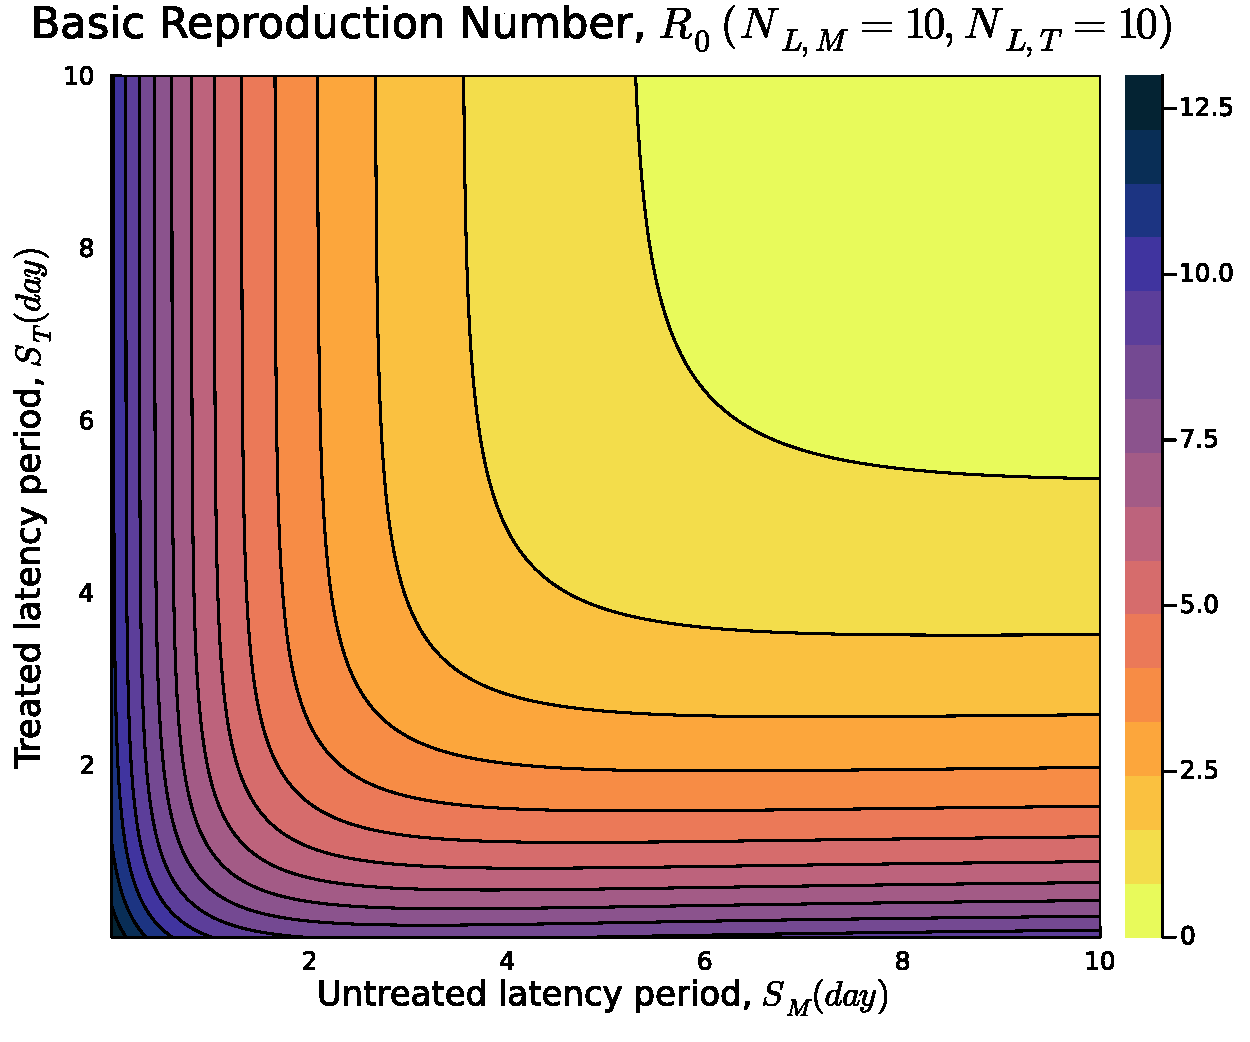
\includegraphics[width=0.3\textwidth]{../../fig/gen_model/R0_periods_SMxST_10x10.pdf}\\
    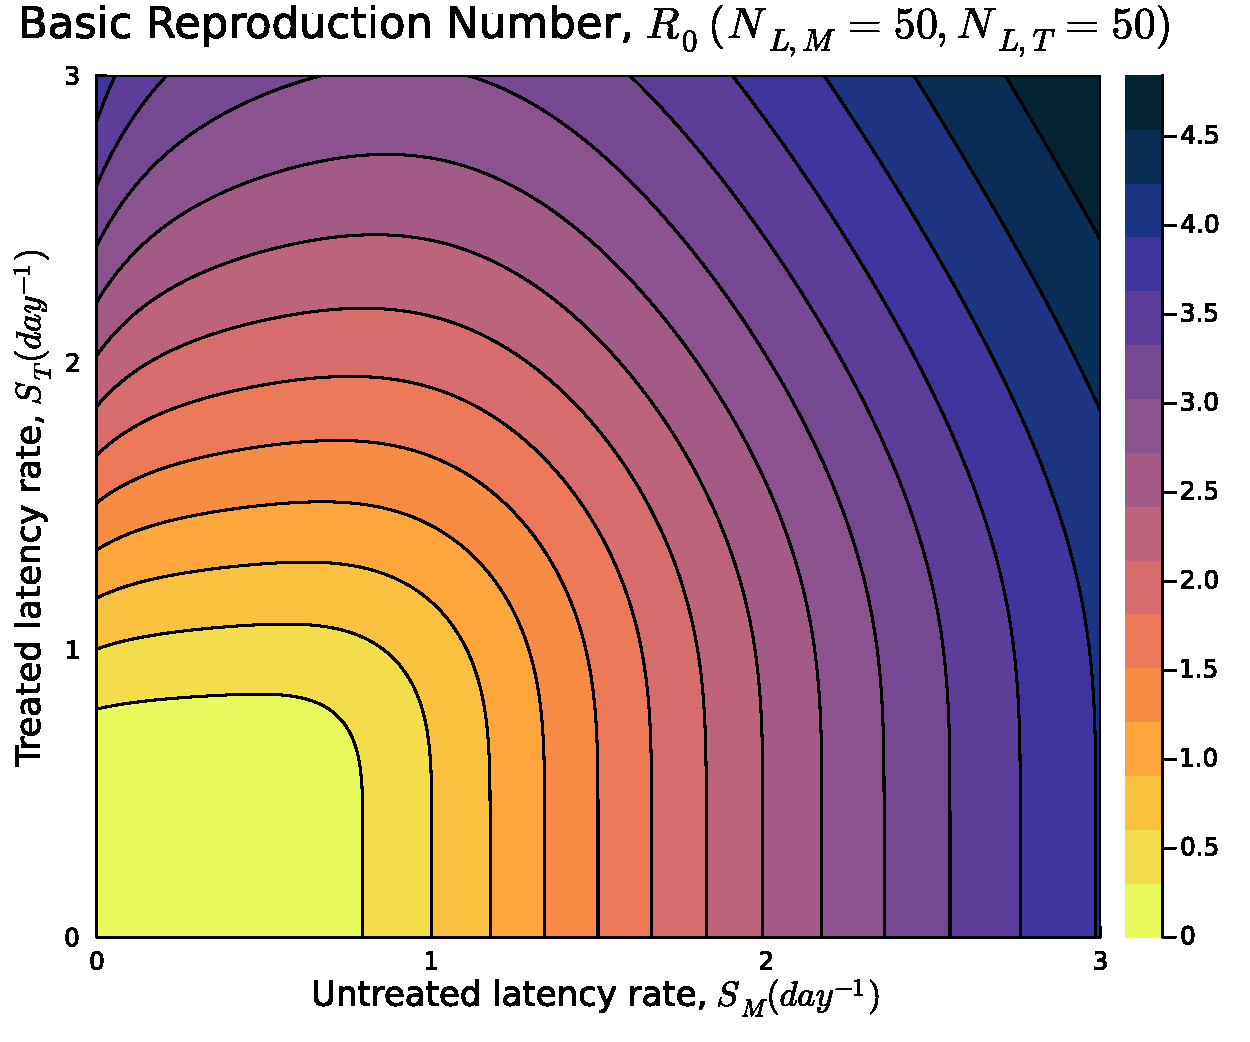
\includegraphics[width=0.3\textwidth]{../../fig/gen_model/R0_rates_SMxST_50x50.pdf}
    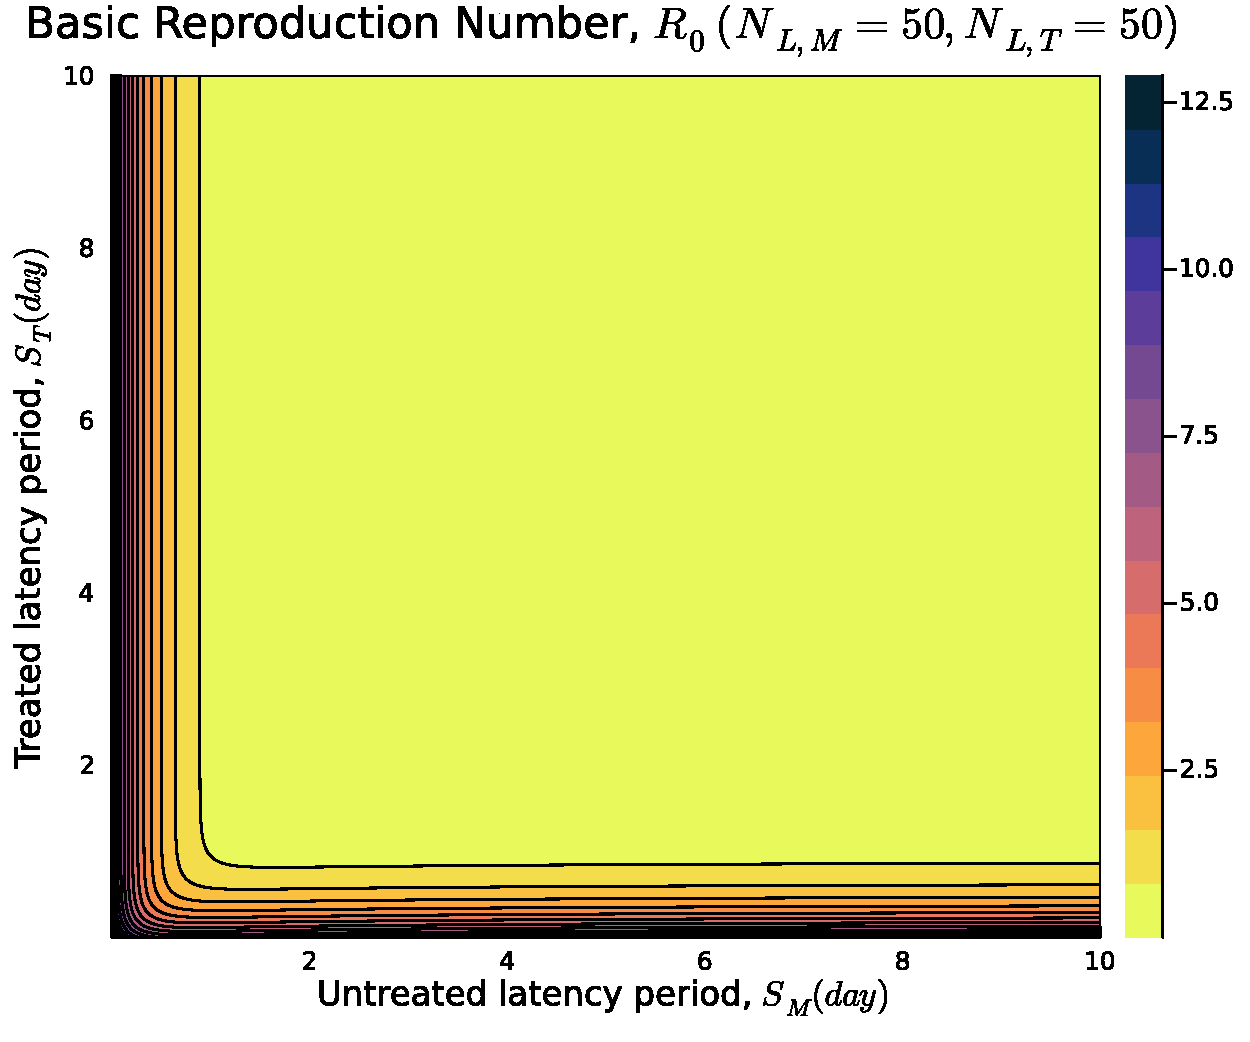
\includegraphics[width=0.3\textwidth]{../../fig/gen_model/R0_periods_SMxST_50x50.pdf}\\
    \caption{\textbf{R0 for latency rate/period parameters.} The left panels shows the basic reproduction number \(R_0\) as a function of the latency rate, while the right panels shows \(R_0\) as a function of the latency period.}
\end{figure}

\begin{figure}[H]
    \centering
    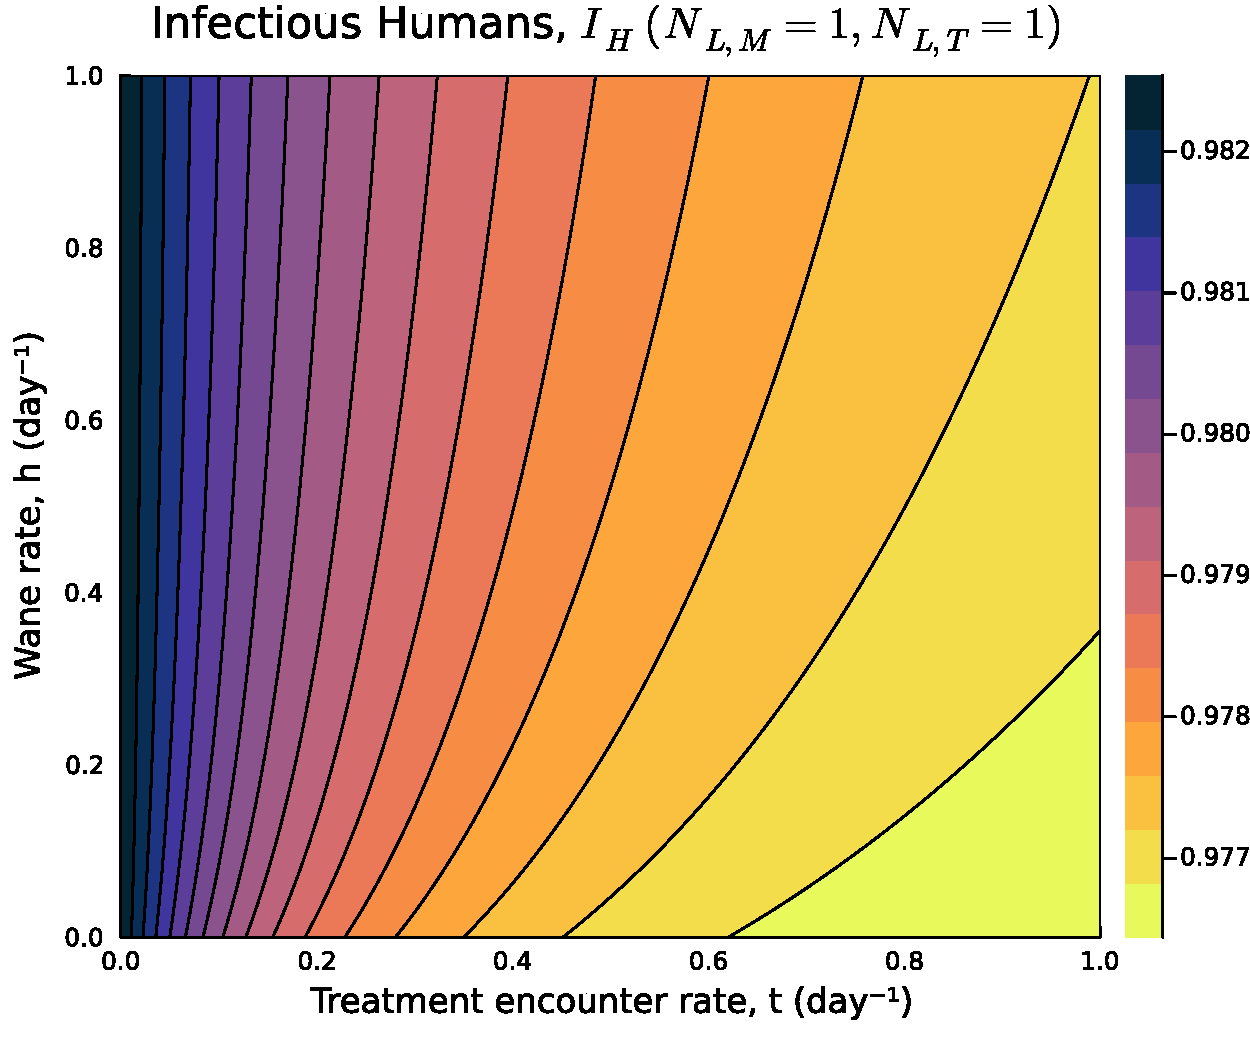
\includegraphics[width=0.3\textwidth]{../../fig/gen_model/IH_rates_txh_1x1.pdf}
    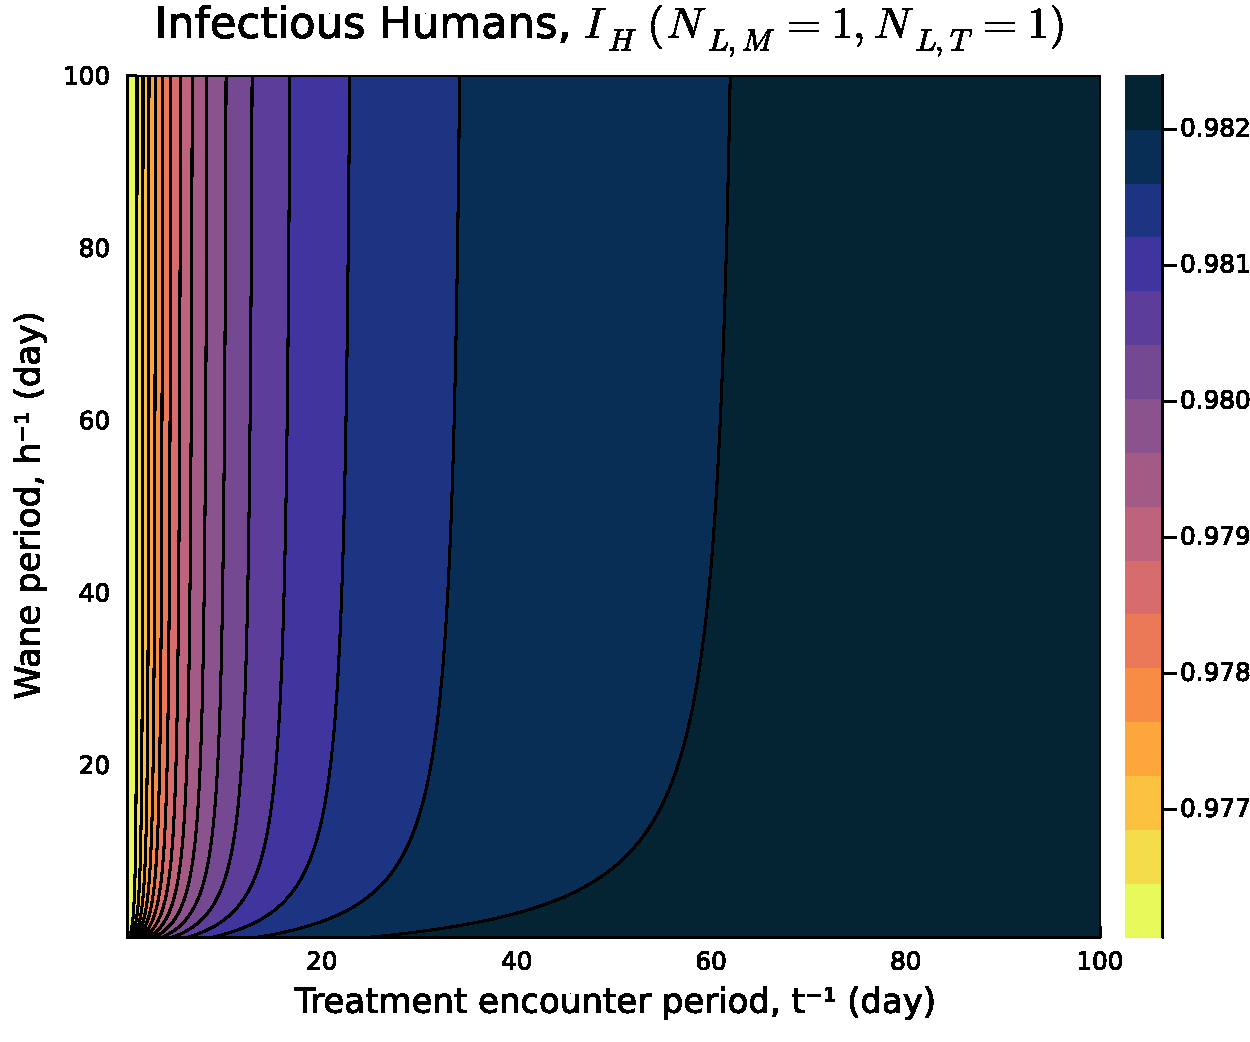
\includegraphics[width=0.3\textwidth]{../../fig/gen_model/IH_periods_txh_1x1.pdf}\\
    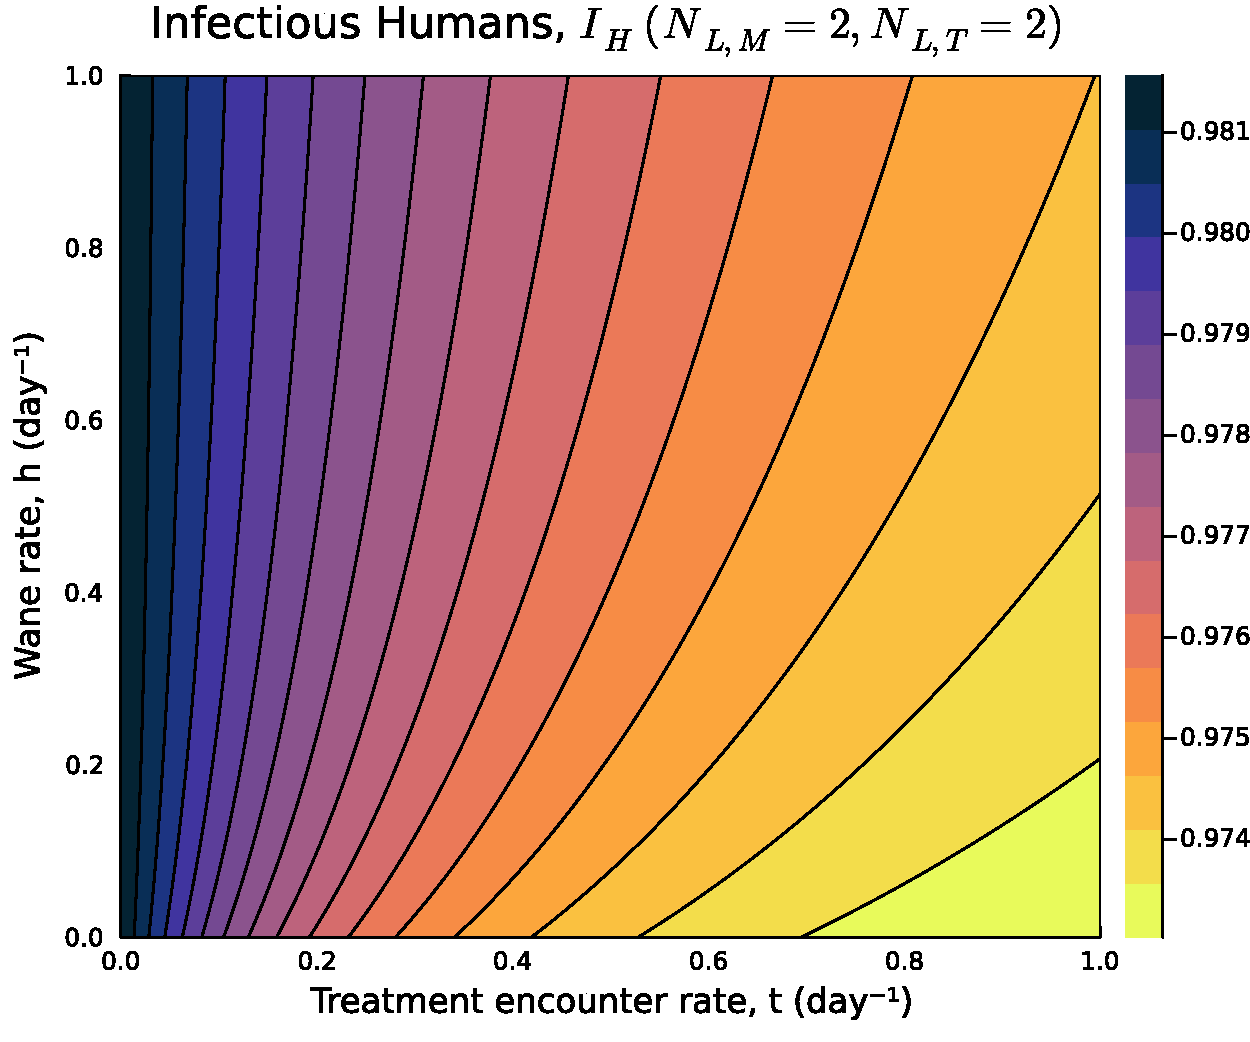
\includegraphics[width=0.3\textwidth]{../../fig/gen_model/IH_rates_txh_2x2.pdf}
    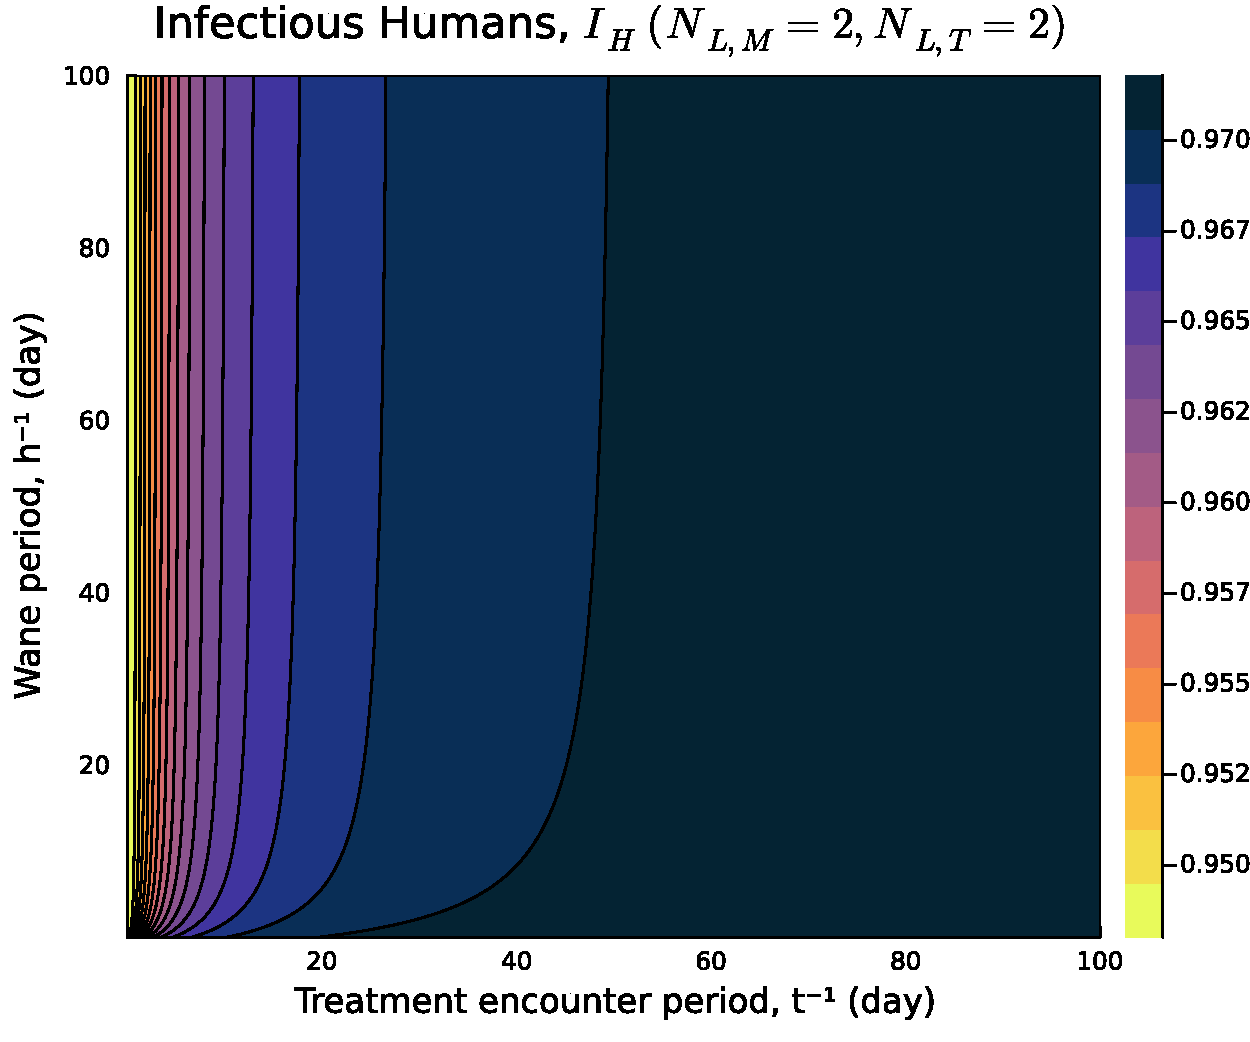
\includegraphics[width=0.3\textwidth]{../../fig/gen_model/IH_periods_txh_2x2.pdf}\\
    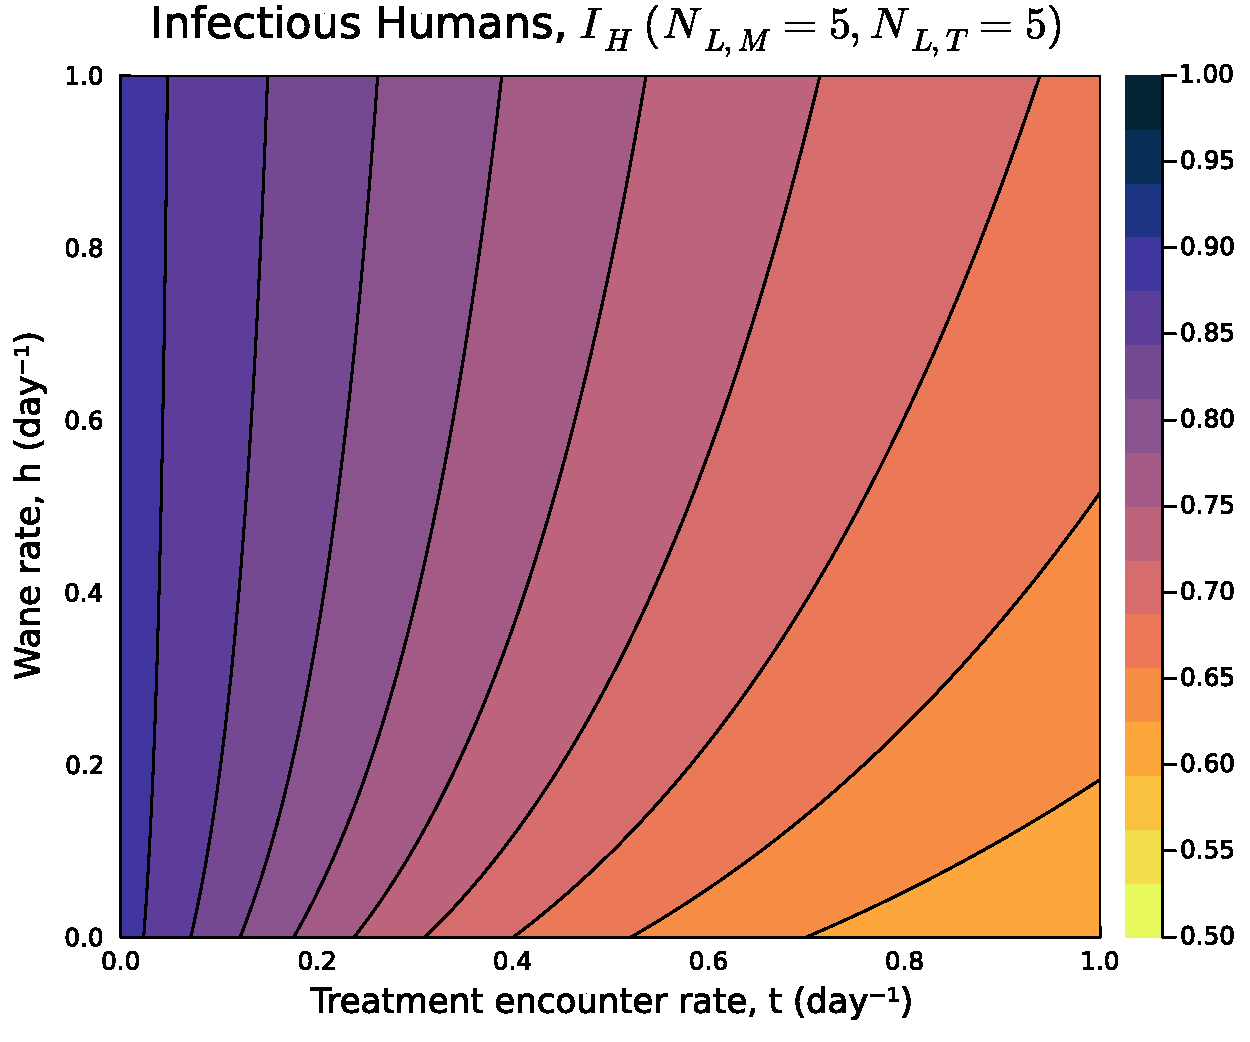
\includegraphics[width=0.3\textwidth]{../../fig/gen_model/IH_rates_txh_5x5.pdf}
    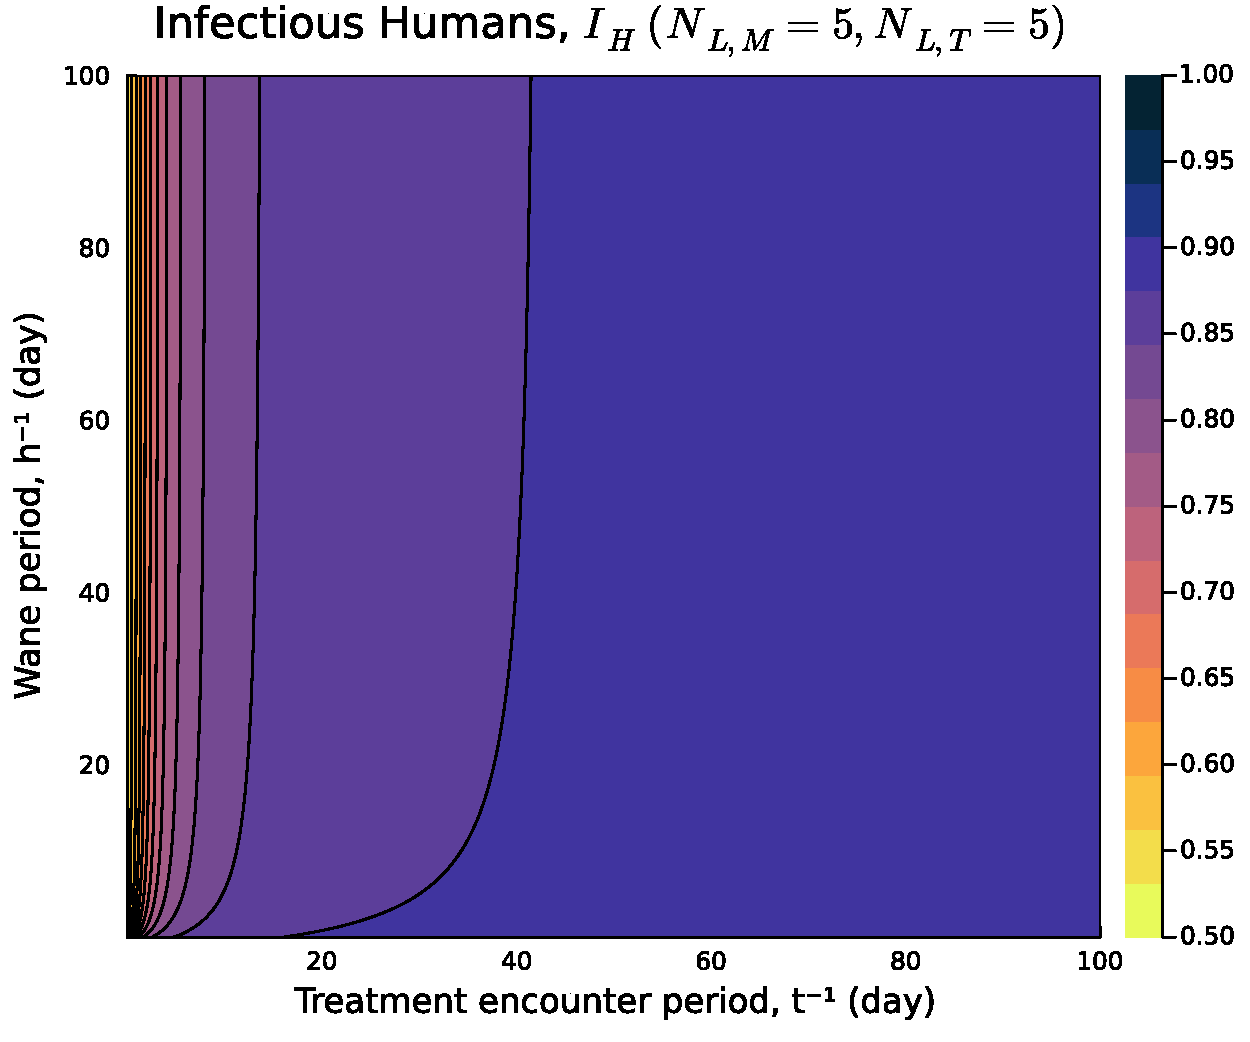
\includegraphics[width=0.3\textwidth]{../../fig/gen_model/IH_periods_txh_5x5.pdf}
    \caption{\textbf{Infections Humans at endemic equilibrium.} The left panels shows the infected humans \(I_H\) as a function of the treatment rate, while the right panels shows \(I_H\) as a function of the treatment period.}
\end{figure}

\begin{figure}[H]
    \centering
    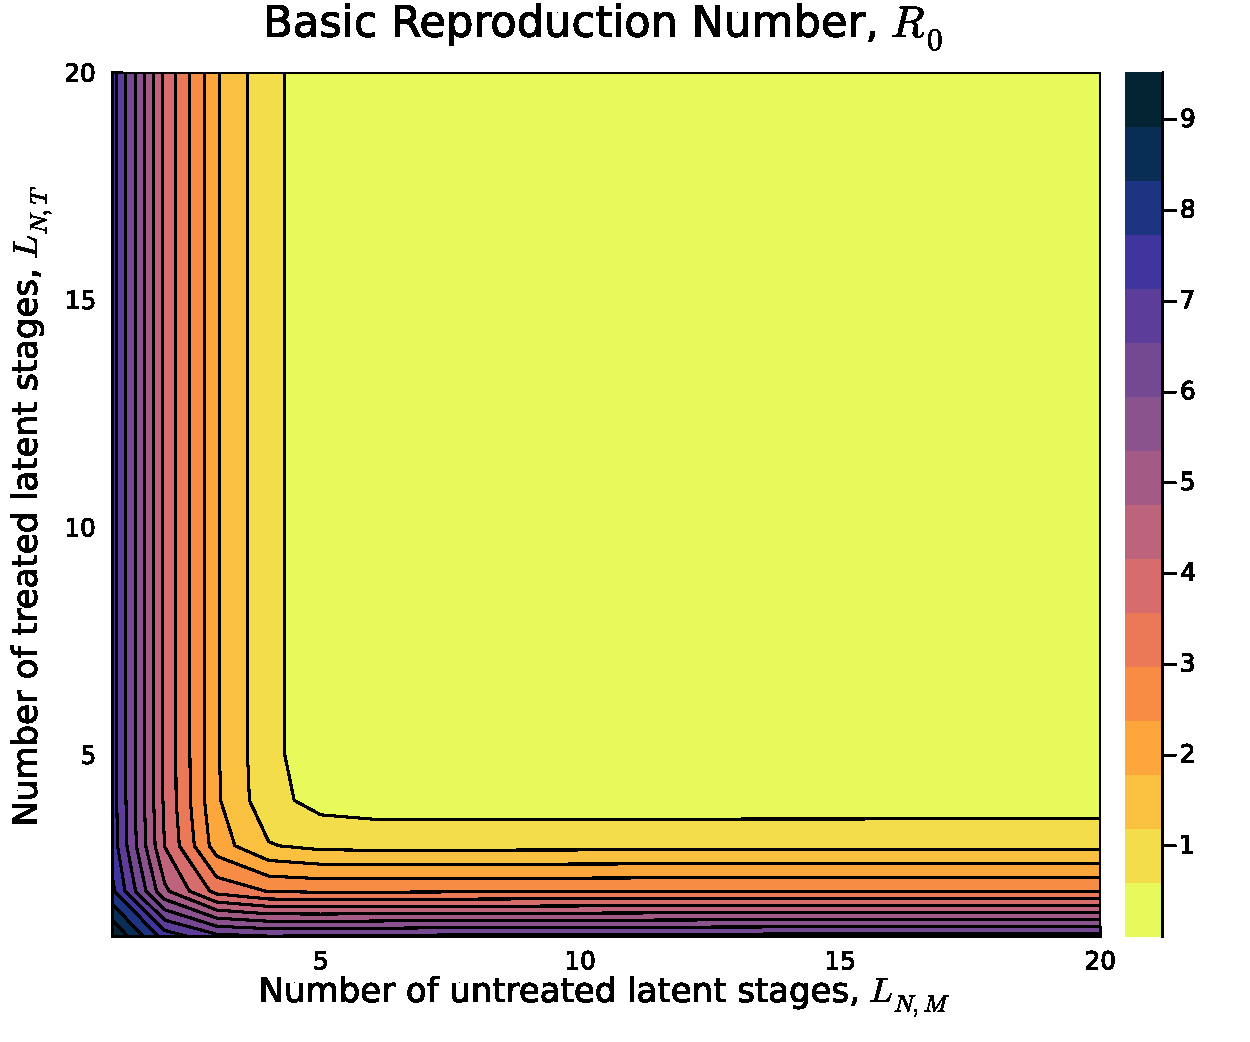
\includegraphics[width=0.3\textwidth]{../../fig/gen_model/R0_NLMxNLT.pdf}
    \caption{\textbf{R0 for number of latent stages.} The basic reproduction number \(R_0\) as a function of the number of latent stages in untreated and treated mosquitoes.}
\end{figure}

\end{document}
